%%
%% Copyright 2019-2024 Elsevier Ltd
%%
%% Version 2.4
%%
%% This file is part of the 'CAS Bundle'.
%% --------------------------------------
%%
%% It may be distributed under the conditions of the LaTeX Project Public
%% License, either version 1.2 of this license or (at your option) any
%% later version.  The latest version of this license is in
%%    http://www.latex-project.org/lppl.txt
%% and version 1.2 or later is part of all distributions of LaTeX
%% version 1999/12/01 or later.
%%
%% The list of all files belonging to the 'CAS Bundle' is
%% given in the file `manifest.txt'.
%%
%% Template article for cas-dc documentclass for
%% double column output.

%\documentclass[a4paper,fleqn,longmktitle]{cas-dc}
\documentclass[a4paper,fleqn]{cas-dc}

%\usepackage[authoryear,longnamesfirst]{natbib}
%\usepackage[authoryear]{natbib}
\usepackage[numbers]{natbib}
\usepackage{rotating}

%%%Author definitions
% \def\tsc#1{\csdef{#1}{\textsc{\lowercase{#1}}\xspace}}
% \tsc{RPK}
% \tsc{ASK}
% \tsc{IAM}
% \tsc{GAM}
% \tsc{MDO}
% \tsc{SSP}
% \tsc{AD}
% \tsc{MTOW}
% \tsc{TLAR}
% \tsc{GDP}
% \tsc{EIS}
% \tsc{JIT}
% \tsc{FD}
% \tsc{SAF}
% \tsc{RCP}
%%%

\begin{document}
\let\WriteBookmarks\relax
\def\floatpagepagefraction{1}
\def\textpagefraction{.001}
\shorttitle{Numerical optimization of aviation decarbonization scenarios}
\shortauthors{I. Costa-Alves et~al.}

\title [mode = title]{Numerical optimization of aviation decarbonization scenarios: balancing traffic and emissions with maturing energy carriers and aircraft technology}


\author[1,2]{Ian Costa-Alves}[type=editor,
                        auid=000,bioid=1,
                        % prefix=Sir,
                        % role=Researcher,
                        orcid=0009-0009-4458-6641]
\cormark[1]
\fnmark[1]
\ead{ian.costa-alves@isae-supaero.fr}
% \ead[url]{www.jkkrishnan.in}

\credit{Conceptualization of this study, Methodology, Software}

%ADdress[1]{, Street 129, 1043 NX Amsterdam, The Netherlands}
\affiliation[1]{organization={Aerodynamics, Energetics and Propulsion Department, ISAE-SUPAERO},
                addressline={10 av. Marc Pélegrin},
                city={Toulouse},
%               citysep={}, % Uncomment if no comma needed between city and postcode
                postcode={31055},
                % state={Kerala},
                country={France}}

\affiliation[2]{organization={Multidisciplinary Optimization Competence Center, IRT Saint Exupéry},
                addressline={3 rue Tarfaya},
                postcode={31400},
                % postcodesep={},
                city={Toulouse},
                country={France}}

\author[1]{Nicolas Gourdain}
\ead{nicolas.gourdain@isae-supaero.fr}

\author[2]{François Gallard}
\ead{francois.gallard@irt-saintexupery.com}


% \fnmark[2]
% \ead{wjh@example.org}
% \ead[URL]{https://www.university.org}

\credit{Data curation, Writing - Original draft preparation}

\author[2]{Anne Gazaix}
% \cormark[2]
% \fnmark[1,3]
\ead{anne.gazaix@irt-saintexupery.com}
% \ead[URL]{www.campus.in}

\author[1,3]{Yri Amandine Kambiri}
\ead{yri-amandine.kambiri@isae-supaero.fr}

\author[3]{Thierry Druot}
\ead{thierry.druot-ext@enac.fr}

\affiliation[3]{organization={Conceptual Airplane Design and Operations, ENAC},
                addressline={7 av. Marc Pélegrin},
                city={Toulouse},
                postcode={31400},
                % state={Orissa},
                country={France}}

% \cortext[cor1]{Corresponding author}
% \cortext[cor2]{Principal corresponding author}
% \fntext[fn1]{This is the first author footnote, but is common to third author as well.}
% \fntext[fn2]{Another author footnote, this is a very long footnote and it should be a really long footnote. But this footnote is not yet sufficiently long enough to make two lines of footnote text.}

% \nonumnote{This note has no numbers. In this work we demonstrate $a_b$ the formation Y\_1 of a new type of polariton on the interface between a cuprous oxide slab and a polystyrene micro-sphere placed on the slab. }

\begin{abstract}
Despite being considered a hard-to-abate sector, aviation’s emissions will play an important role in long-term climate mitigation of transportation. The introduction of low-carbon energy carriers and the deployment of new aircraft in the current fleet are modeled as technology-centered decarbonization policies, while supply constraints in targeted market segments are modeled as demand-side policies. Shared Socioeconomic Pathways (SSPs) are used to estimate trend-mitigation traffic demand and to limit the sectoral consumption of electricity and biomass. Mitigation scenarios are formulated as optimization problems, and three applications are demonstrated: no-policy baselines, single-policy optimization, and scenario-robust policies. Results show that the choice of energy carrier is highly dependent on assumptions regarding aircraft technology and the background energy system. Across all SSP-based scenarios, emissions peak by around 2040, but achieving alignment with the Paris Agreement requires either targeted demand management or additional low-carbon energy supply. The use of gradient-based optimization within a multidisciplinary framework enables the efficient resolution of these nonlinear, high-dimensional problems while reducing implementation effort.
\end{abstract}

% \begin{graphicalabstract}
% 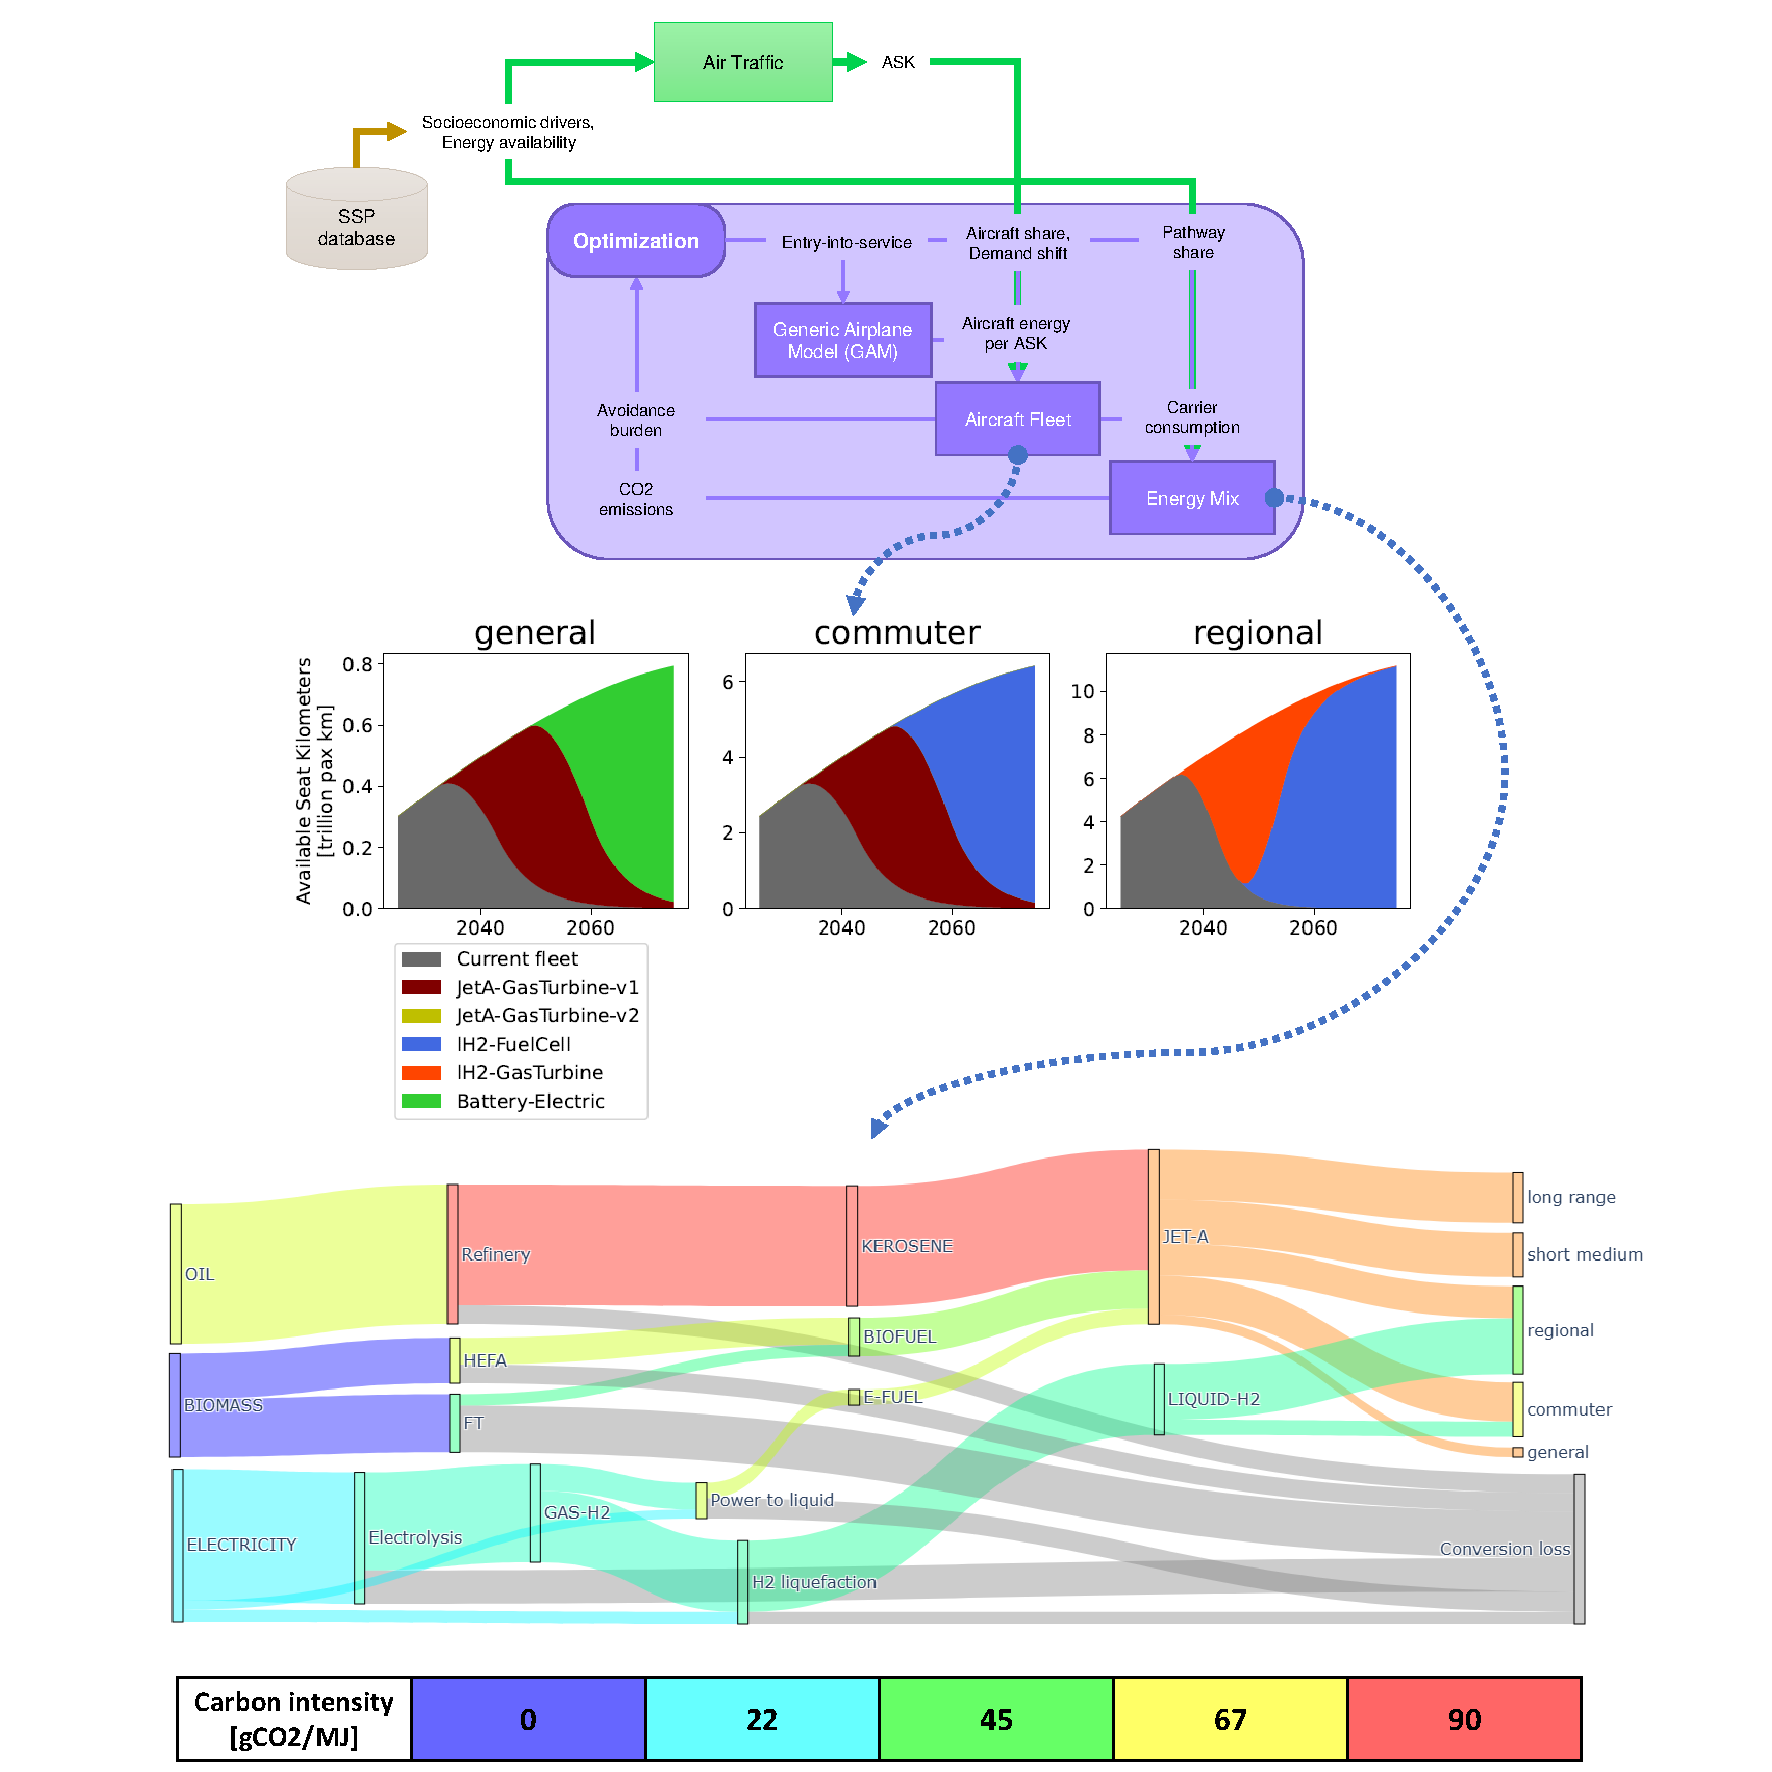
\includegraphics[width=\textwidth]{figs/graphical_abstract.pdf}
% \end{graphicalabstract}

\begin{highlights}
\item Optimization framework links SSP scenarios with detailed aircraft technology;
\item Fleet replacement and demand saturation leads to emissions peak around 2040;
\item Impact of alternative aircraft requires extending analysis beyond 2050;
\item Respecting +2°C carbon budgets requires demand caps or extra energy availability;
\item Policy optimization was prohibitive without speedups from numerical methodology.
\end{highlights}

\begin{keywords}
Multidisciplinary Optimization \sep Low-carbon fuels \sep Aircraft design \sep Integrated Assessment Models \sep Shared Socioeconomic Pathways
\end{keywords}


\maketitle


\begin{nomenclature}
\begin{deflist}[AAAA] %[AAAA] if you have 4 letters max for example
\defitem{AD}\defterm{Automatic Differentiation}
\defitem{ASK}\defterm{Available Seat Kilometers}
\defitem{ATJ}\defterm{Alcohol-to-Jet}
\defitem{BtL}\defterm{Biomass-to-Liquid}
\defitem{EIS}\defterm{Entry-Into-Service}
\defitem{FD}\defterm{Finite Differences}
\defitem{FT}\defterm{Fischer-Tropsch}
\defitem{GAM}\defterm{Generic Airplane Model}
\defitem{GDP}\defterm{Gross Domestic Product}
\defitem{HEFA}\defterm{Hydroprocessed Esters and Fatty Acids}
\defitem{IAM}\defterm{Integrated Assessment Model}
\defitem{IPCC}\defterm{Intergovernmental Panel on Climate Change}
\defitem{JIT}\defterm{Just-In-Time}
\defitem{LH2}\defterm{Liquid hydrogen}
\defitem{MDO}\defterm{Multidisciplinary Optimization}
\defitem{PtL}\defterm{Power-to-Liquid}
\defitem{RCP}\defterm{Representative Concentration Pathway}
\defitem{RPK}\defterm{Revenue Passenger Kilometers}
\defitem{SAF}\defterm{Sustainable Aviation Fuel}
\defitem{SSP}\defterm{Shared Socioeconomic Pathways}
\defitem{TLAR}\defterm{Top Level Aircraft Requirements}
\end{deflist}
\end{nomenclature}

\section{Introduction}
\label{sec:intro}

Air transportation is often considered a hard-to-abate sector, because carbon-free commercial aircraft are not readily available, and the production of alternative energy carriers to fossil kerosene on a global scale requires significant amounts of biomass and low-carbon electricity to meet the growing demand \cite{becken_implications_2023}. However, the sector will play a critical role in long-term climate mitigation of transportation \cite{girod_global_2012}.

Several key energy carriers have emerged as potential substitutes of conventional kerosene, such as synthetic kerosene (from biomass-to-liquid or power-to-liquid pathways), liquid hydrogen, ammonia, liquid natural gas, ethanol, methanol, and batteries \cite{ansell_review_2023}. Among these, only synthetic kerosene can be used in today’s fleet without aircraft re-deisgn. Current engines are limited by certification to a 50 \% mixing ratio with conventional kerosene, but there is ongoing advances on the operation with 100 \% Sustainable Aviation Fuels (SAF) \cite{full-saf}. There is, however, among industry roadmaps a systematic over-reliance on SAF deployment, which could require 9 \% of global renewable electricity and 30 \% of sustainably available biomass by 2050 \cite{becken_implications_2023}.

Compared to ground and marine transportation vehicles, aircraft are more weight sensitive because they must generate lift in order to remain airborne. Increasing mass leads to an increase in induced drag, which further increases the structural mass to support extra loads, leading to more drag, and so on. This snowball effect is a central phenomenon in the conception of aircrafts \cite{raymer_aircraft_2018}, which means that estimating energy consumption is a fundamentally coupled problem. Alternative aircraft designs, flying with different energy carriers, may display higher energy consumption and/or limited payload and ranges compared to conventional jet-fueled planes, due to low specific energy (batteries) or due to the need for heavier cryogenic fuel tanks (liquid hydrogen).

% \footnote{Long-range aircraft, for example, can have more than 45 \% of its Maximum Take-Off Weight (MTOW) as fuel weight, meaning the vehicle will be much heavier at take-off than it would need, simply because it needs to carry extra fuel that will be spent in the end of its mission.}

\begin{quote}
    "Since the IPCC’s Fifth Assessment Report (AR5) there has been a growing awareness of the need for demand management solutions combined with new technologies, such as the rapidly growing use of electromobility for land transport and the emerging options in advanced biofuels and hydrogen-based fuels for shipping and aviation." \cite[][Executive Summary]{transport_ar6_wg3}
\end{quote}

Integrated Assessment Models (IAM) are the tools used to simulate the evolution of the coupled climate-energy-land system from socioeconomic assumptions on climate mitigation and adaptation. Since the publication of the Shared Socioeconomic Pathways (SSP) \cite{riahi_shared_2017}, great improvements have been made in the detail given to transportation modes within global mitigation. The modeling of aviation within IAM's, has shown how demand-side measures may play an important role in keeping temperature increase between 1.5 and 2° C above preindustrial levels \cite{sharmina_decarbonising_2021}, but also how the incorporation of synthetic kerosene and the deployment of new aircraft with alternative energy carriers (such as hydrogen and biofuels) can also play a significant role in reaching stringent targets \cite{napp_role_2019, speizer_integrated_2024}.

However, the detail these studies have concerning the fleet composition and how they are arranged within market segments is limited, e.g., \cite{speizer_integrated_2024} considers kerosene, electric, and hydrogen aircraft to have similar energy consumption even for long-haul (where electric is unfeasible, and hydrogen is less efficient), while \cite{napp_role_2019} accounts for lower efficiencies for hydrogen, it does so with a singular value applied for the entire fleet. The performance of hydrogen aircraft is highly dependent on their range and the cryogenic tank technology \cite{adler_hydrogen-powered_2023}, which can lead to increased energy consumption \cite{icct_hydrogen} or limited operation in terms of payload and ranges \cite{icct_fuelcell}. For electric aircraft, this is even more pronounced as the battery weight significantly shortens the maximum achievable range and payload, making these aircraft only suited to regional flights \cite{icct_electric}.

Sectoral specific scenarios can account for this either with a detailed network of Origin-Destination pairs \cite{grewe_evaluating_2021, eaton_regional_2024, hoelzen_h2-powered_2025}, or by separating the traffic into market segments according to flown distance. A review of sectoral aviation scenarios \cite{delbecq_sustainable_2023} shows that methodologies may differ regarding: traffic evolution, mitigation levers, inclusion of non-CO2 effects, and resource consumption. Employing open-source tools, such as the AeroMAPS framework \cite{planes_aeromaps_2023}, to simulate these types of scenarios can be greatly beneficial to explicit modeling assumptions and finding a common ground for high-level decision making.

From a technological perspective, it is important to map the range of components that are required for novel system architectures. In the context where many of such components are still at immature technologies and require significant allocation of resources to develop, quantifying upper and lower bounds associated to each component is paramount to compare architectural choices in terms of system-level performances \cite{kirby_forecasting_1999} and in end-point metrics, such as financial returns \cite{de_weck_technology_2022}. Regarding climate mitigation, determining the best "carbon-neutral" propulsion architecture choice for each flight is subject of recent interest \cite{adler_energy_2025}, but rely on the strong assumption of dedicated renewable electricity to power aviation, which may be supply constrained.

\subsection{Research positioning}

Global IAM's lack technology and fleet detail concerning aviation emissions, while industry roadmaps and technology assessments rely on strong assumptions of abundant renewable energy. We propose to bridge these together using optimization to endogenously chose appropriate timing and market penetration of conventional and alternative aircraft concepts, subject to a background scenario using the AR6 scenario database \cite{ar6_database}.

These policy scenarios are nonlinear, with many variables due to disaggregation (per market and technologies), and time-dependent (high-dimensional arrays). In practice, even the simpler policy optimization problems may: fail to converge under gradient-free nonlinear optimizers, display significant online linearization cost or offline implementation burden for gradient-based optimization. The numerical methodology aspect of this paper is therefore a central contribution, reducing policy optimization time from 1.5 hours to a single minute on a conventional laptop.

This work builds on the literature of aviation climate mitigation scenarios by linking sectoral mitigation with a background system based on the Shared Socioeconomic Pathways (SSP). Socioeconomic drivers are used to estimate future traffic volumes, based on the assumption that historical trends on traffic growth from personal income and population growth remain unchanged. Biomass and electricity consumed by scenarios are limited by using the concept of a fair share of global production that is allocated to the sector, which avoids over-consumption that can be detrimental to other economic sectors. Fleet and technology detail are also incorporated by modeling conceptual design and possible Entry-Into-Service (EIS) of 4 aircraft propulsion architectures, each linked to component-level performances that mature over time.

This methodology was introduced in \cite{costaalves-isabe}, which addressed the exploration of technology-based decarbonization scenarios with optimization algorithms. Novel developments include the incorporation of voluntary and price-based demand avoidance strategies, the timing of introduction of new technologies, and scenario-robust optimizations.

It is important to note that the generated scenarios are considered as decarbonization scenarios rather than climate mitigation scenarios, because non-CO2 emissions are unaccounted for. While these effects can make up for more than half of aviation's contribution to global warming in the 2000-2018 period \cite{lee_contribution_2021}, there are still significant uncertainties concerning their estimation, especially when considering novel propulsion systems, for which little data is available. Furthermore, because of the short-lived nature of these warming effects, the debate on which metrics to use for comparing them to CO2 is still ongoing \cite{megill_alternative_2024}.

While the usage of optimization within IAM's is not new \cite{nordhaus_optimal_1992, barrage_policies_2023, gcam-2019, witness}, there are several limitations with the tools used to solve them, which often imply a simplification of the problem: reducing time resolution, linearization of the problem \cite{huppmann_messageix_2019}, or even simplification of two-way couplings \cite{jgcricassandra_2024}. Multidisciplinary Optimization (MDO) frameworks can offer methods that allow for: formalizing the coupled problem within optimization routines, and using gradient-based algorithms, which allows nonlinear optimization to scale well despite increasing number of variables. On this methodological front, the present work also contributes to the formulation of optimal mitigation policies, and to alleviate the main drawback of using IAM's with MDO: the extra implementation burden, which is dealt with by using libraries with automatic differentiation capabilities.

The paper is organized as follows: first the quantitative models used are briefly described, along with the methodology and implementation behind optimal scenario formulation; then the principal results from proposed scenarios are presented, analyzed, and compared with current aviation scenarios based on IAMs; the shortcomings of models are made explicit in the limitations section; a critical view on the results and implications from the modeled future are addressed in the discussion; finally, the conclusion summarizes the contributions and key findings of the study.

\begin{figure*}
	\centering
	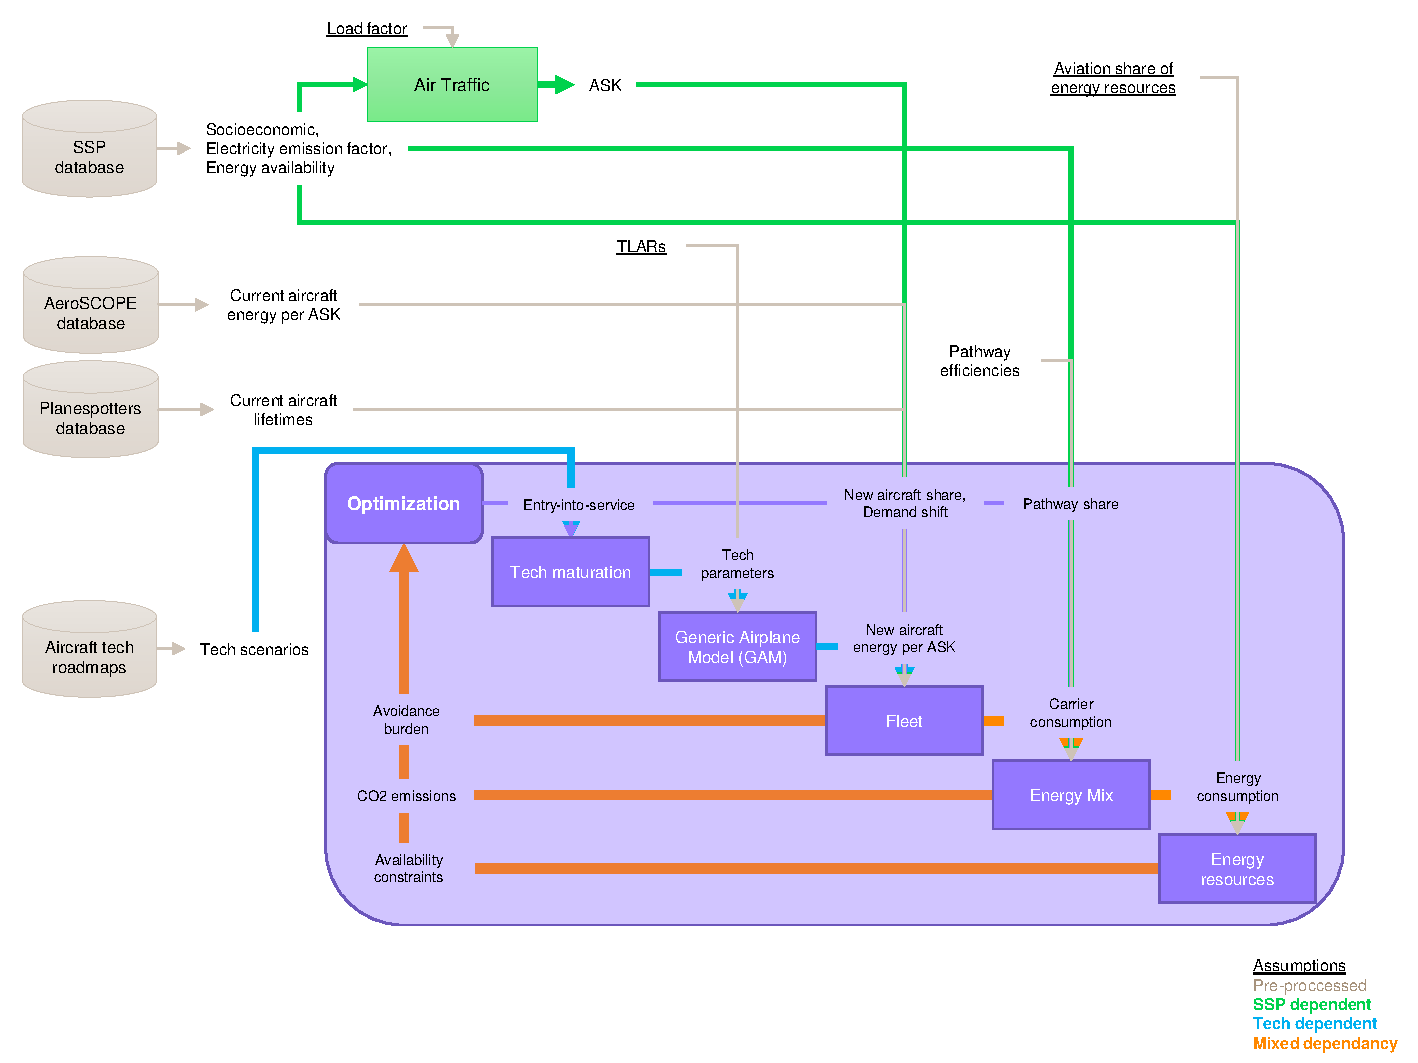
\includegraphics[width=\textwidth]{figs/models_detailed.pdf}
	\caption{Conceptual view of the optimization process and data-flow between modeled disciplines.}
	\label{fig:models}
\end{figure*}

\section{Methods}
\label{sec:methods}

An overview of the data-flow between the model disciplines is presented in Figure \ref{fig:models}. Before the optimization loop starts, the chosen global scenario determines the evolution of socioeconomic drivers (population and economy) and energy system (global production of biomass and electricity, and emission factor of grid electricity). Then, iteratively a set of policy variables is chosen (when and how much to deploy new aircraft, how much to produce of energy pathways, how much of trend traffic to avoid) and the simulation models are evaluated for estimating objective, and constraints for a given optimization formulation.

The numerical methods employed to accelerate optimization for nonlinear and time-dependent policy analysis were crucial to enable fast multi-scenario analysis. These include: automatic model coupling, constrained gradient-based optimization algorithms, automatic differentiation, vectorization, and compilation.

\begin{table*}[htbp]
\centering
\setlength{\tabcolsep}{2pt}
\rotatebox{90}{
    \begin{minipage}{\textheight}
    \caption{Main assumptions for of the model disciplines.}
\begin{tabular}{p{0.1\textwidth}|p{0.5\textwidth}|p{0.3\textwidth}}
\toprule
\textbf{Model discipline} & \textbf{Assumptions} & \textbf{Limitations}  \\
\midrule
Policy controls &
Policy variables act on fleet replacement (per aircraft per market) and energy production shares (per pathway), the low-demand formulation also includes a cap in supply (per market). Controls evolve gradually in time subject to a linear delay. &
Time-delayed share-based control creates instability under rapid production volume changes.\\
\midrule
Air traffic demand &
Future trend Revenue Passenger Kilometers (RPK) demand estimated based on scenario-dependent population and income per capita \cite{ar6_database}. Demand grows with income, but is assumed to saturate at around 2700-4300 pax-km/capita (scenario-dependent) and represented via sigmoidal (logistic-type) functions calibrated on historical data. The supply, in terms of Available Seat Kilometers (ASK), is then estimated using a quadratic load factor \cite{planes_aeromaps_2023, planes_simulation_2021} that grows from 84.4 \% (2019) to 92 \% (2075). &
Prospective analysis uses logistic functions outside range of calibrated data, problematic for estimating saturation levels of developing countries. Global aggregation ignores regional disparities. Price elasticity not coupled with energy costs.
\\
\midrule
Current aircraft &
The initial fleet composition and performance are fixed and calibrated to historical data \cite{salgas_aeroscope, planespotters}. Fleet parameters (efficiency, lifetime) are exogenous and differentiated by market segments, but may vary due to technology assumptions. &
Potential mismatch between current efficiency (aggregated by flight distance) and aircraft lifetimes (aggregated by number of seats).
\\
\midrule
New aircraft &
Generic Airplane Model (GAM) \cite{kambiri_energy_2024} for conceptual design of future aircraft with conventional and alternative propulsion architectures, such as: (i) conventional kerosene turbofan, (ii) liquid-hydrogen turbofan, (iii) liquid-hydrogen fuel-cell and electric motors, and (iv) battery-electric aircraft. Aircraft are designed for market-specific missions, and deployed by Entry-Into-Service (EIS) year, which are also optimization variables (per market per aircraft). Technology maturing is incorporated with assumptions component-level performances (structures, batteries, cryogenic tanks, fuel cell, ...) that varies in time and according to technology assumptions, reducing energy consumption at later EIS. &
TLAR fixed within markets (size, speed, altitude not optimized). Cryogenic tank efficiency fixed across markets, ignoring size dependency \cite{adler_hydrogen-powered_2023, ati_cryogenic}. Gas turbine weight and consumption assumed identical for kerosene and hydrogen \cite{mourouzidis_abating_2024}.
\\
\midrule
Fleet replacement &
Current aircraft is replaced by new aircraft types, designed specifically for market range. Replacement is gradual with market-specific lifetimes of 15.3-33.8 years (variable with technology assumptions). &
Airlines may operate aircraft at shorter distances than designed mission, increasing fuel consumption beyond modeled values.
\\
\midrule
Energy mix &
Aviation energy demand may be supplied by a mix of different energy carriers (Jet-A fuel, Batteries, Liquid-hydrogen), each of them being produced by different production pathways (fossil kerosene, biofuels, e-fuels, electrolysis, ...). Well-to-wake (WTW) lifecycle emissions are considered for all carriers, with constant in time carbon intensities for kerosene and biofuels \cite{jing_understanding_2022, NEULING201854}, while electricity-based pathways have emission intensities calculated based on process efficiencies \cite{wallington_green_2024} and scenario-dependent grid emission intensity. &
No differentiation between biomass types (all pathways compete for same resource). PtL consumption assumes only Direct Air Capture as source for carbon, concentrated CO2 sources are not considered \cite{drunert_ptl}.
\\
\midrule
Constraints &
Feasibility is evaluated with: initialization constraints (each aircraft must be feasible by EIS), and path-wise constraints (current fleet retirement per market, pathway-mix per carrier, fair share of biomass and electricity consumption), the low-demand formulation also includes an end-time constraint (cumulative emissions). &
Fair shares of global production allocated to aviation estimated with grandfathering approaches based on energy consumption.
\\
\midrule
Objectives &
Minimize cumulative emissions (trend formulation), or minimize discounted relative price increase due to supply-cap (low demand formulation). & Simplified modeling of relative price increase with constant price elasticities among markets. \\
\bottomrule
\end{tabular}
\label{tab:model_assumptions}
    \end{minipage}
}
\end{table*}

\subsection{Background scenarios}

The Shared Socioeconomic Pathways (SSP) were introduced between IPCC's 5th and 6th Assessment Report (AR5 and AR6) as a way to bridge the socioeconomic dimension of mitigation into climate assessments \cite{riahi_shared_2017}. These scenarios are formulated based on qualitative stories first, which define high-level assumptions that steer IAM simulations into different possible futures regarding economic development, demographics, energy production, and land-use. Each SSP is created from a storyline to represent a consistent underlying logic to the depth of socioeconomic changes that societies are expected to have:

\begin{itemize}
    \item SSP1: Sustainability – Taking the Green Road (Low challenges to mitigation and adaptation): “The world shifts gradually, but pervasively, toward a more sustainable path, emphasizing more inclusive development that respects perceived environmental boundaries. Consumption is oriented toward low material growth and lower resource and energy intensity” \cite{ssp1}.
    \item SSP2: Middle of the Road (Medium challenges to mitigation and adaptation): “The world follows a path in which social, economic, and technological trends do not shift markedly from historical patterns. Global and national institutions work toward but make slow progress in achieving sustainable development goals” \cite{ssp2}.
    \item SSP5 Fossil-fueled Development – Taking the Highway (High challenges to mitigation, low challenges to adaptation): “This world places increasing faith in competitive markets, innovation and participatory societies to produce rapid technological progress and development of human capital as the path to sustainable development. At the same time, the push for economic and social development is coupled with the exploitation of abundant fossil fuel resources and the adoption of resource and energy-intensive lifestyles around the world” \cite{ssp5}.
\end{itemize}

After the adoption of the Paris Agreement, studies focused on the investigation of pathways limiting warming to 1.5°C \cite{ipcc_wg3_an3} in the context of the Special Report on Global Warming of 1.5°C (SR1.5). From then until AR6, significant work has been done in improving the modeling of energy and transportation technologies, and in multi-model studies covering scenarios from extrapolation current policy trends and the implementation of NDCs, all of them are made available in the AR6 scenario database \cite{ar6_database}, which is used to provide for scenario-dependent inputs.

From each baseline SSP, mitigation scenarios are introduced by incorporating varying mitigation strategies and are named according to a target radiative forcing by the end of the century, these are made to match scenario emissions to a Representative Concentration Pathway (RCP), which are used in the analysis carried by the IPCC Working Groups 1 and 2. These scenarios are then incorporated by main modeling groups, each resposible for one IAM, forming an SSP-RCP-IAM matrix (see \cite{ipcc_wg3_an3}).

\subsection{Models}

An overview of the models and assumptions behind scenario generation is provided in Table \ref{tab:model_assumptions}, for a more detailed explanation on assumptions, model equations, comparison with related works, and calibration methodology refer to the section 1 of the Supplementary Information (SI).

In earlier studies \cite{costaalves-isabe}, models primarily aimed to link SSP scenario data and aircraft design routines within an aviation system model, through a direct re-implementation of AeroMAPS equations \cite{planes_aeromaps_2023}. The new models and numerical methods developed in this work will subsequently be re-incorporated into AeroMAPS.

\begin{figure*}
    \centering
    
\includegraphics[width=\textwidth]{figs/rpk_ssps.pdf}
    \caption{Historical evolution and modeled future global RPK demand from socioeconomic drivers linked to SSP scenarios. Results are compared with \cite{franz_wide_2022}. Explicitly incorporating per-capita demand saturation (current model) yields much lower traffic levels in the long term, when compared with models based on the extrapolation of short term income elasticities.}
    \label{fig:global-demand}
\end{figure*}

The energy inputs consumed to meet the necessary final energy carrier production and the emissions generated are estimated from process efficiencies, direct emissions from pathway production and grid electricity emission factor linked to a global scenario. In the present model, each biofuel pathway competes for the same biomass feedstock, considering direct emissions and process efficiencies as an average of the different feedstock-specific processes \cite{NEULING201854}. However, this approach represents a simplified view, since each biofuel pathway can actually consume specific feedstocks, such as energy crops (competing with food production), oil-based feedstocks and wastes. For example, HEFA biofuels can be obtained from oil-based feedstocks (such as jatropha and camelina), but also from used cooking oil. The final climatic impact of biofuels also depends on potential land use change, especially in the case of competition with food production \cite{yang_sustainable_2025}.

The modeling of costs (energy, aircraft, operations) is outside the scope of this paper. Under the current production system, the price of alternative energy carriers is higher than that of fossil kerosene \cite{salgas_cost_2023, salgas_marginal_2024}, but this gap is expected to decrease in the near future due to scaling of production and due to carbon pricing \cite{dray_cost_2022}, especially in scenarios with ambitious climate targets.

\subsubsection{Air Traffic Demand}

In order to account for the phases of growth, maturation and saturation observed in aviation demand \cite{vedantham_aircraft_1994}, a generalized logistic function is used to estimate trend per-capita demand from per-capita income. This model explicitly accounts for saturation of per-capita transport demand as per-capita incomes grow, differently to the approach in most IAMs, which rely on extrapolations \cite{franz_wide_2022} or assumptions of constant income elasticity \cite{kim_gcam_2006, gcam-2019}.

Figure \ref{fig:global-demand} shows the recent history and SSP scenario future evolution of Population and GDP per capita, and also the recent history and modeled future global RPK demand. SSP2 follows the historically calibrated logistic function, demand grows with varying pace due to income growth, but stabilizing at around 3000 passenger-kilometers per capita. SSP1 displays high initial growth due to income, but stabilizes demand sooner and 90 \% lower than trend; while for SSP5 growth is sustained at even higher pace, and stabilize at much higher levels of around 4300 passenger-kilometers per capita, 50 \% higher than trend. For comparison, crossing AeroSCOPE \cite{salgas_aeroscope} and World Bank \cite{world_bank} averaged 2019 traffic per capita for multiple countries: India is 198, China 902, Brazil 959, \textbf{World 1377}, Japan 2669, France 3561, Germany 3718, and USA 6974.

\begin{figure*}
    \centering
    
\includegraphics[width=\textwidth]{figs/aircraft_prospective_energy.pdf}
    \caption{Expected passenger efficiency (inverse energy consumption) of prospective aircraft with technology available by Entry-Into-Service. Color-code is used to differentiate among aircraft architectures, filled between the upper and lower limit for the technology scenarios, solid line shows Lower technology scenario, dotted line shows Mid technology scenario. The grey horizontal lines shows the values initialized for the current technology, estimated based on the 3 quartiles (Lower: 1st quartile, Mid: median, Upper: 3rd quartile) of 2019 flights within market distance-bands \cite{salgas_aeroscope}.}
    \label{fig:aircraft-performance}
\end{figure*}

As highlighted in the assessment by Frank \textit{et al.} \cite{franz_wide_2022} when estimating demand there is also the need of endogenizing SSP narratives beyond accounting for scenario-specific GDP and population growth, a proposition is also made for incorporating \textbf{voluntary demand restraint} (for SSP1 scenarios) \textbf{or incentives} (in SSP5 scenarios) as well as an extra policy measure of market-specific demand caps for dealing with strict carbon budget constraints. Comparing these results with the ones generated by the present work, SSP1 shows a very close agreement both in terms of per-capita traffic as for total demand, SSP2 shows close agreement up until 2070, after that the logistic model employed yields lower per-capita traffic than Franz's model, with declining income elasticities. This disagreement is further intensified in SSP5, even with the higher stabilization traffic levels.

\subsubsection{Aircraft Design}

Figure \ref{fig:aircraft-performance} shows the expected design performance of aircraft design architectures depending on prospective technology scenario. Energy consumption of new designs are compared with the 3 quartiles of 2019 commercial flights operated within the category distance bands, obtained from the AeroSCOPE dataset \cite{salgas_aeroscope}.

\textbf{Conventional aircraft}

In general, new conventional gas turbine designs, powered by Jet-A perform better than the mean 2019 fleet, and this gap is wider over smaller distances. The diverging expectations in weight reduction expectations, yield a variation in the energy consumption of these designs depending on the chosen technology scenario, but this variation is relatively small compared to that of alternative designs.

\textbf{Electric aircraft}

Due to the low specific energy of batteries compared to other energy carriers, electric aircraft are still limited in range. Performance varies greatly with technology scenario, due to variation of batteries, electric motors, and power electronics.

Low technology yields that feasible designs in the general market are only possible around 2050. With Mid and Upper technology, respectively, feasibility can be achieved by 2037 and 2032 in the general market, and by 2046 and 2038 in the commuter. By 2060, with Upper technology, electric aircraft is the most efficient for the general market.

\textbf{Hydrogen aircraft}

Hydrogen aircraft are feasible across all markets regardless of EIS, both for architectures that burn hydrogen in gas turbines as for using them with fuel-cells and electric motors. Technology scenario affects them more than conventional aircraft, but less than electric. The sensibility regarding technology scenario is due to the gravimetric efficiency of liquid fuel tanks, but the fuel cell architecture displays higher sensitivity, also due to electric motors and fuel cells (both in terms of efficiency and specific power).

With Lower technology, burning hydrogen in gas turbines is more efficient than using fuel cell for all markets, regardless of  EIS. In the general and commuter market, as early as 2030 both are already more efficient than the reference 2019 aircraft. In the regional market, this shift happens by early 2034 and 2042, respectively. In the short-medium, by 2044 and 2050. But neither of them are able to reach 2019 efficiencies in the long-range even by 2050.

With Mid technology, fuel cells surpass combustion around 2040, a bit earlier for shorter distances and a bit later for longer distances. Within the time-frame, both are able to surpass 2019 efficiencies, but neither are able to surpass the efficiency of turbofan architectures.

Finally, with Upper technology hydrogen combustion is able to reach the Lower efficiency of conventional designs. Also with Upper technology scenario, fuel cells are the most efficient option among architectures, except for the general market, but this supposes switching membranes with low temperature operation to high temperature \cite{ati_fuelcell}.

\subsection{Optimization formulation}

Optimal mitigation policies are formulated as the general nonlinear programming problem. Two formulations of optimal mitigation scenarios are proposed: one relying on minimizing cumulative emissions by \textbf{supplying for trend demand}, while changing energy carriers and aircraft within the global fleet, here called trend formulation; and other that \textbf{partially avoids trend traffic} and minimizes the relative ticket price increase in order to align to a target cumulative emissions, here called low-demand formulation.

The optimization variables consist of aircraft market penetration parameters (per aircraft and per market), energy mix parameters (shares of energy production per pathway per period), and, for the low-demand formulation, the supply cap parameters (share of avoided demand per market per period). Entry-Into-Service is bounded between 2035 and 2060 for all aircraft types, except for the first generation of conventional aircraft (which can be launched and deployed as soon as 2030), the energy mix variables between 0 and 1, and $SR$ between 0 and 0.9 (at least 10 \% of the trend demand is satisfied at each market).

The optimization constraints applied to all scenarios consist in limiting the sum of the control inputs among aircraft types for each market to 1, limiting the share of pathway production to positive values among each produced energy, and limiting the consumption of biomass and electricity to a fixed fair share of the global production. Also, in the case where scenarios add electric aircraft to the fleet, an extra constraint on aircraft energy consumption is added to ensure designs are feasible by EIS.

In the trend formulation the objective function is the cumulative CO2 emissions. In the low-demand formulation, cumulative emissions are constrained, and the objective is the time-discounted mean burden of demand aversion (see Equation 10 in the SI).

Numerical optimization is performed with the SLSQP Algorithm \cite{kraft1988software}, using forward-mode AD to obtain the gradients of objective and constraints. Forward-mode is chosen over reverse-mode, or backpropagation, due to the larger memory footprint when multiple constrains are involved (which is the case here) \cite{blondel2024}.
% In reverse-mode, a backpropagation strategy is used, requiring to store intermediate computations in the memory and AD will re-trace the computation graph, this however yields a .
% One way to overcome this, is to perform time integration of constraint violation, reducing the dimension of outputs to differentiate, therefore lowering memory and computational footprint associated with backpropagation. When compared to forward-mode, this approach can lead to faster differentiation, but at the expense of the optimization convergence when multiple constrains are involved (which is the case here).
% Time-integration of constraint violation is essentially viewed as a \texttt{sum} over a vectorized \texttt{if($g\le value$)} statement, which is non-differentiable. When AD is applied over this operation it will compute a gradient that only accounts for the instants where the condition is true. This wrong approximation of the gradient of $\mathbf{g}$ leads to an optimization that takes more iterations to reach the same level of convergence, or even fails to converge in some cases.

\subsubsection{Robustness to background scenario}

The robustness to the background scenario was also performed as a policy optimization problem. First a formulation must be chosen (results demonstrate the case for the trend formulation) and is performed in a multi-scenario simulation. The objective of the optimization problem is then considered as the mean of policy objectives under the scenario ensemble.

The optimization variables are then divided into two sets: one that is kept fixed among all scenarios (the aircraft mix variables), and one that may be specific to each scenario (the energy mix variables). This allows to ensure the robustness of the choice of aircraft mix while allowing for each scenario to individually optimize the energy production system in order to respect their respective availability constraints.

\begin{table*}[width=\linewidth,cols=7,pos=h]
    \caption{Benchmark over a Drop-in policy optimization with trend formulation. Performed using a single Intel(R) Core(TM) i7-10850H CPU core with 2.70 GHz, as the mean of 3 repetitions, varying technology assumptions. The objective (cumulative CO2 emissions) is normalized by the 3\% of the 2°C carbon budget.}
    \centering
    \begin{tabular}{c|c|c|c c c|c}
    \toprule
     Method & Algorithm & Gradient-based & Iterations & Total time (s) & Speedup & Objective value \\
    \midrule

    Standard (FD) & \multirow{3}{*}{SLSQP} & \multirow{3}{*}{Yes} & X & X & X & X \\
    FD + JIT & &  & 91 & 69.3 & 87 & 1.72 \\
    JAX version &  &  & 86 & 53.2 & 114 & 1.72 \\
    % \toprule
    % Speedup & & & 24 & 81 & - \\
    % \bottomrule
    \midrule
    Standard & \multirow{2}{*}{COBYLA} & \multirow{2}{*}{No} & 1852 & 6052 & - & 1.75 \\
    JAX version &  &  & 1898 & 51 & 119 & 1.75 \\
    % \toprule
    % Speedup & & & - & 119 & - \\
    \bottomrule
    \end{tabular}
    \label{tab:optimization}
\end{table*}

\subsection{Numerical Methodology}

% \subsection{Differential Programming for Multidisciplinary Optimization}

% Knowledge of new mitigation technology and climate sciences evolves constantly, therefore models also need to be continuously improved to account for new findings. As a consequence, the implementation burden associated to adding, modifying and extending models should be kept low.

The optimization of mitigation scenarios requires libraries that allow for: assembly and integration of numerous heterogeneous models; scaling with high-dimensional variables, due primarily to the disagregation among periods, technologies, and markets; minimal extra implementation when incorporating or modifying models.

Multidisciplinary Optimization (MDO) frameworks are classically used to optimize or improve a given design under various constraints \cite{mdobook}, it offers practical methods to handle model integration and coupling. Efficient optimization under high-dimension can also be achieved by using gradient-based algorithms, but their use often implies an extra burden due to the manual implementation of the derivatives of objective and constraints with regards to optimization variables. GEMSEO is an open-source Python software to automate multidisciplinary processes \cite{gallard_gems_2018}, which provided the following features that were used in the present study: automatic handling of coupled derivatives, automatic assembly of complex MDO processes based on dependency graphs, interfaces to optimization algorithms, results visualization, data storage.

Differential Programming, on the other hand, is commonly used for machine learning and scientific computing research. This programming paradigm allows for the Automatic Differentiation (AD) of lines of code. The use of AD for MDO can significantly reduce implementation burden associated to efficient high-dimension optimization. JAX is a library for array-oriented numerical computation, with capabilities for AD and just-in-time (JIT) compilation \cite{jax2018github}, enabling high-performance scientific computing in multiple hardware configurations (CPU, GPU, and TPU).

GEMSEO-JAX \cite{gemseo_jax} is an open-source plug-in that was developped by the authors to bridge JAX programs into a GEMSEO process.

\subsection{Computational gains}
\label{subsec:gains}

\begin{table}[width=\columnwidth,cols=3,pos=h]
    \caption{Benchmark over a single scenario computation and linearization. Performed using a mean of 50 repetitions in a single Intel(R) Core(TM) i7-10850H CPU core with 2.70 GHz.}
    \centering
    \begin{tabular}{c|c c}
    \toprule
    Method & Computation (s)  & Linearization (s)\\
    \midrule
    Standard (FD) & 372.7 & 362.6 \\
    JAX version & 0.45 & 0.48 \\
    \midrule
    Speedup & 830 & 749 \\
    \bottomrule
    \end{tabular}
    \label{tab:execution-linearization}
\end{table}

To evaluate the simulation gains offered by a Differential Programming paradigm, we first compare execution times over full scenario optimizations, then over a single computation and linearization.

\begin{table*}[htbp]
\centering
% \setlength{\tabcolsep}{2pt}
\rotatebox{90}{
    \begin{minipage}{\textheight}
    \caption{Overview of simulated scenarios and their assumptions regarding: the background scenario, personal demand saturation, presence of traffic aversion policies, optimization objective, energy carriers included, the share of global energy production allocated to aviation, and the technology scenarios. In case multiple background scenarios, the objective is the mean among realizations. The demand saturation indicates storyline-specific assumptions on the stabilization level of per-capita demand. In presence of extra price-based traffic aversion, the objective is the minimization of relative ticket price increase. The energy carriers included are subject to variable Entry-Into-Service, and are limited to a fixed share of global production of biomass and electricity. Finally, the technology scenarios are determinant of the aircraft technology parameters, impacting the performance of new aircraft designs, driving the choice of which architectures to deploy.}
    \footnotesize
    \begin{tabular}{c|c|c c|c|c c|c}
    \toprule
    \multirow{2}{*}{Scenario name} & \multirow{2}{*}{Background scenario} & \multicolumn{2}{c|}{Demand} & Policy objective & \multicolumn{2}{c|}{Energy} & \multirow{2}{*}{Tech scenarios} \\
    & & Saturation & Traffic aversion & ($\min$) & Carriers & \% of production &\\
    \midrule
    Baseline SSP1 & SSP1-1.9 & Trend -10\% & - & Cumulative CO2 &  Jet-A (fossil) & - & Lower, Mid, Upper\\
    Baseline SSP2 & SSP2-2.6 & Trend & - & Cumulative CO2 &  Jet-A (fossil) & - & Lower, Mid, Upper\\
    Baseline SSP5 & SSP5-4.5 & Trend +50\% & - & Cumulative CO2 & Jet-A (fossil) & - & Lower, Mid, Upper\\
    \midrule
    Drop-in trend & SSP2-2.6 & Trend & - & Cumulative CO2 &  Jet-A (fossil+SAF) & 5.0 & Lower, Mid, Upper\\
    Drop-in availability & SSP2-2.6 & Trend & - & Cumulative CO2 &  Jet-A (fossil+SAF) & 8.6 & Lower, Mid, Upper\\
    Drop-in low-demand & SSP2-2.6 & Trend & \checkmark & \textbf{Rel. price increase} &  Jet-A (fossil+SAF) & 5.0 & Lower, Mid, Upper\\
    \midrule
    Breakthrough trend & SSP2-2.6 & Trend & - & Cumulative CO2 & Jet-A (fossil+SAF), LH2, Battery & 5.0 & Lower, Mid, Upper\\
    Breakthrough availability & SSP2-2.6 & Trend & - & Cumulative CO2 & Jet-A (fossil+SAF), LH2, Battery & 8.6 & Lower, Mid, Upper\\
    Breakthrough low-demand & SSP2-2.6 & Trend & \checkmark & \textbf{Rel. price increase} & Jet-A (fossil+SAF), LH2, Battery & 5.0 & Lower, Mid, Upper\\
    \midrule
    Scenario-robust trend & SSP2-1.9, 2.6, and 3.4 & Trend & - & \textbf{Mean} cumulative CO2 & Jet-A (fossil+SAF), LH2, Battery & 5.0 & Mid\\
    Scenario-robust low-demand & SSP2-1.9, 2.6, and 3.4 & Trend & \checkmark & Min rel. price increase \\
    \bottomrule
    \end{tabular}
    \label{tab:scenarios}
    \end{minipage}
}
\end{table*}

In Table \ref{tab:optimization}, entire scenario optimization is performed with varying optimization algorithm, differentiation strategies, and compilation. Gradient-based algorithms not only require far fewer iterations for convergence but also achieve higher objective precision, confirming their advantages for high-dimensional problems \cite{perez_pyopt_2012}. Using an uncompiled model with standard Finite Differences (FD) was prohibitive due to memory demands; JIT compilation makes FD feasible yet still less efficient—both in iteration count and runtime—than forward-mode AD. Overall, using JAX yields speedups of up to two orders of magnitude for both algorithms tested.

In Table \ref{tab:execution-linearization} the computation compares compares how long one single scenario computation takes to complete with (JAX version) and without (standard) JIT compilation, and the time required to linearize objectives and constraints. JAX introduces an initial overhead of roughly 38\,s due to compilation; this is excluded from single computation comparisons but included in full-optimization timings. Once compiled, JAX achieves speedups of up to three orders of magnitude.

For context, a single scenario simulation using a restricted subset of AeroMAPS models \cite{planes_aeromaps_2023} (default bottom-up setup without offsetting, non-CO\textsubscript{2}, or cost models) takes 1.29\,s, about three times slower than the present approach. This comparison should be interpreted cautiously, as the modeling scopes differ substantially: AeroMAPS includes freight, non-CO\textsubscript{2} effects, and cost models, but omits aircraft design routines and links between traffic growth and socioeconomic drivers.

\section{Scenario Results}
\label{sec:results}


\begin{figure*}
    \centering

    (a) Baseline:

    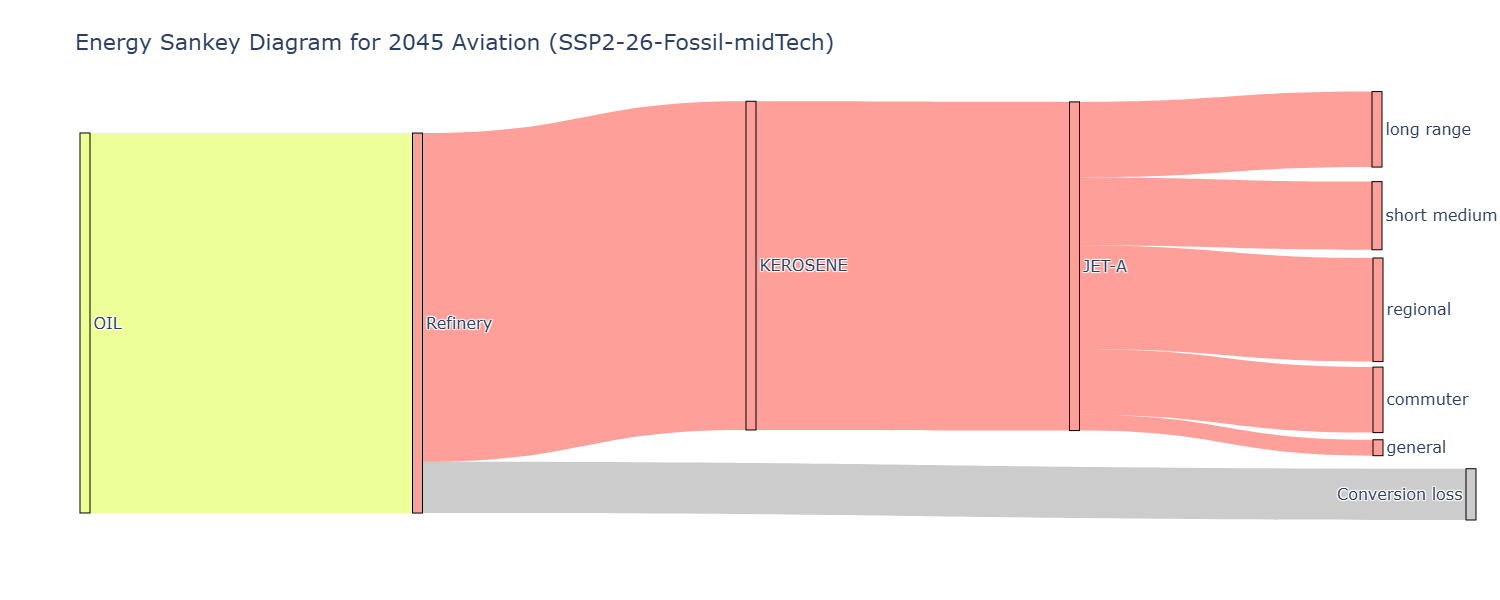
\includegraphics[clip, trim=0cm 0cm 0cm 2cm, width=0.9\textwidth]{figs/sankey-baseline.png}

    (b) Drop-in:

    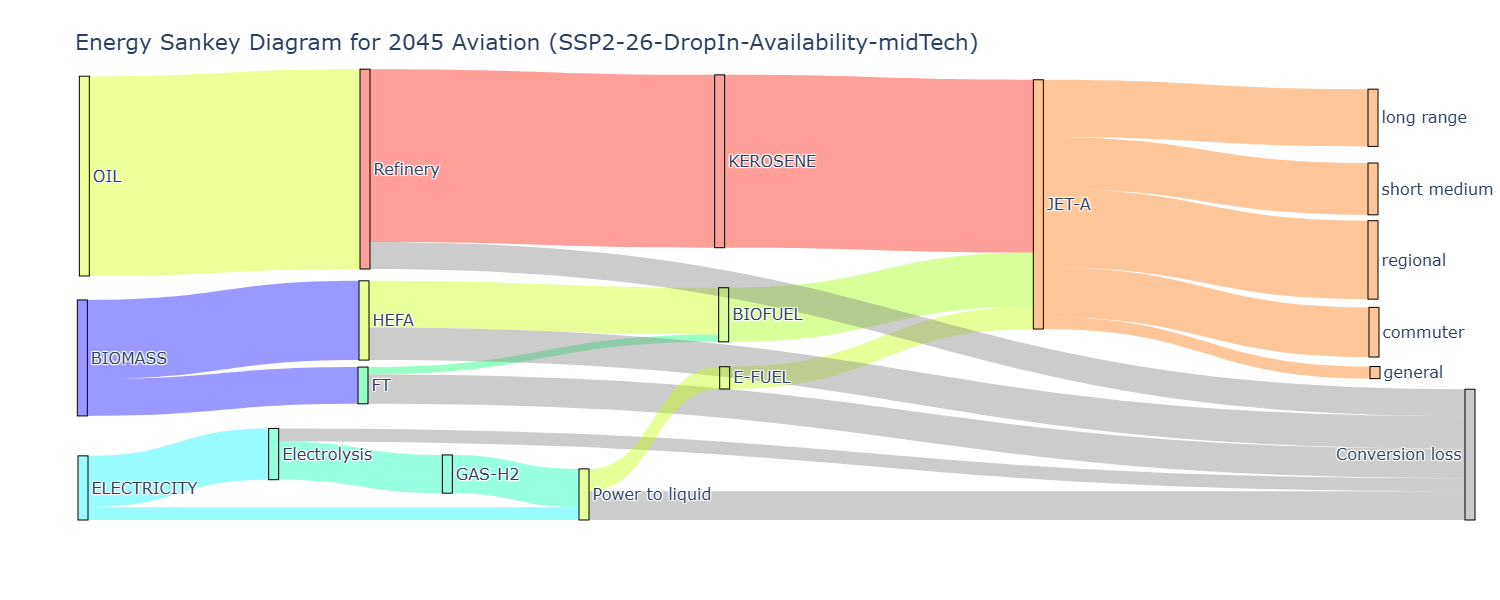
\includegraphics[clip, trim=0cm 0cm 0cm 2cm, width=0.9\textwidth]{figs/sankey-dropin-a.png}

    (c) Breakthrough:

    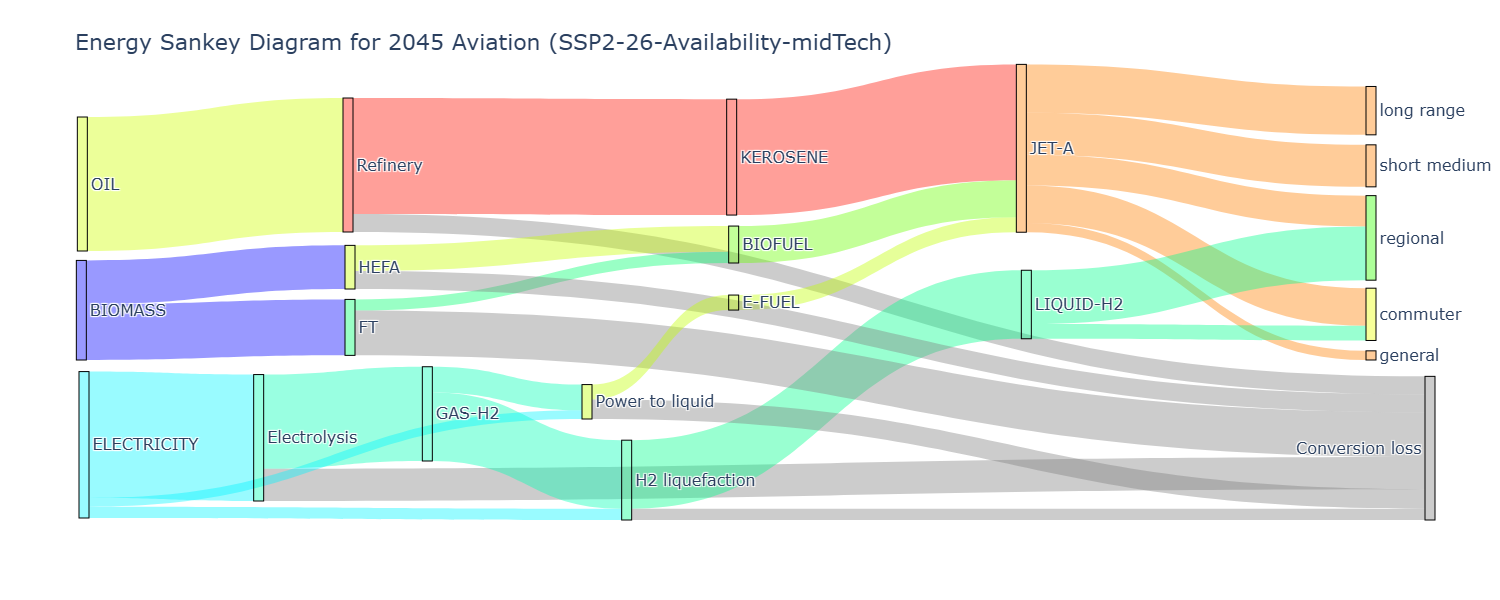
\includegraphics[clip, trim=0cm 0cm 0cm 2cm, width=0.9\textwidth]{figs/sankey-break-a.png}

    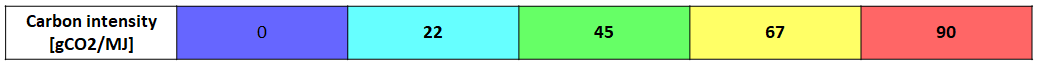
\includegraphics[width=0.7\textwidth]{figs/sankey-scale.png}

    \caption{Comparison of energy production sankey diagram for global aviation by 2045 for SSP2 scenarios: (a) Baseline, (b) Drop-in, and (c) Breakthrough. These also assume extra energy availability, and Mid aircraft technology.}
    \label{fig:sankey}
\end{figure*}

Several policy scenarios are simulated using the numerical optimization methods presented, these are summarized in Table \ref{tab:scenarios}.

We start with the \textbf{baseline} no-policy scenarios (SSP1, 2, and 5), where two new generations of conventional aircraft are launched, and their entry-into-service and deployment is optimized to minimize cumulative emissions, while consuming only fossil kerosene. The sensibility to maturing aircraft technology is also explored with 3 technology scenarios affecting: energy consumption of current aircraft, fleet replacement lifetimes, and energy consumption of new aircraft (Fig. \ref{fig:aircraft-performance}).

Then the mitigation scenarios are explored using SSP2 as the baseline. The Drop-in \textbf{trend} mitigation scenarios also introduce incorporation of biofuel and electrofuel (SAF) in the Jet-A blend, and constraint the sectoral consumption of electricity and biomass to 5.0 \% of the global supply. The Drop-in \textbf{availability} mitigation scenario increases the sectoral consumption to 8.6 \%. And the Drop-in \textbf{low-demand} mitigation scenario keeps trend consumption, but avoids traffic in order to fulfill an additional constraint on the total cumulative emissions. As the baseline scenarios, these are also explored with 3 technology scenarios.

\begin{figure*}
    \centering
    (a) Baseline:

    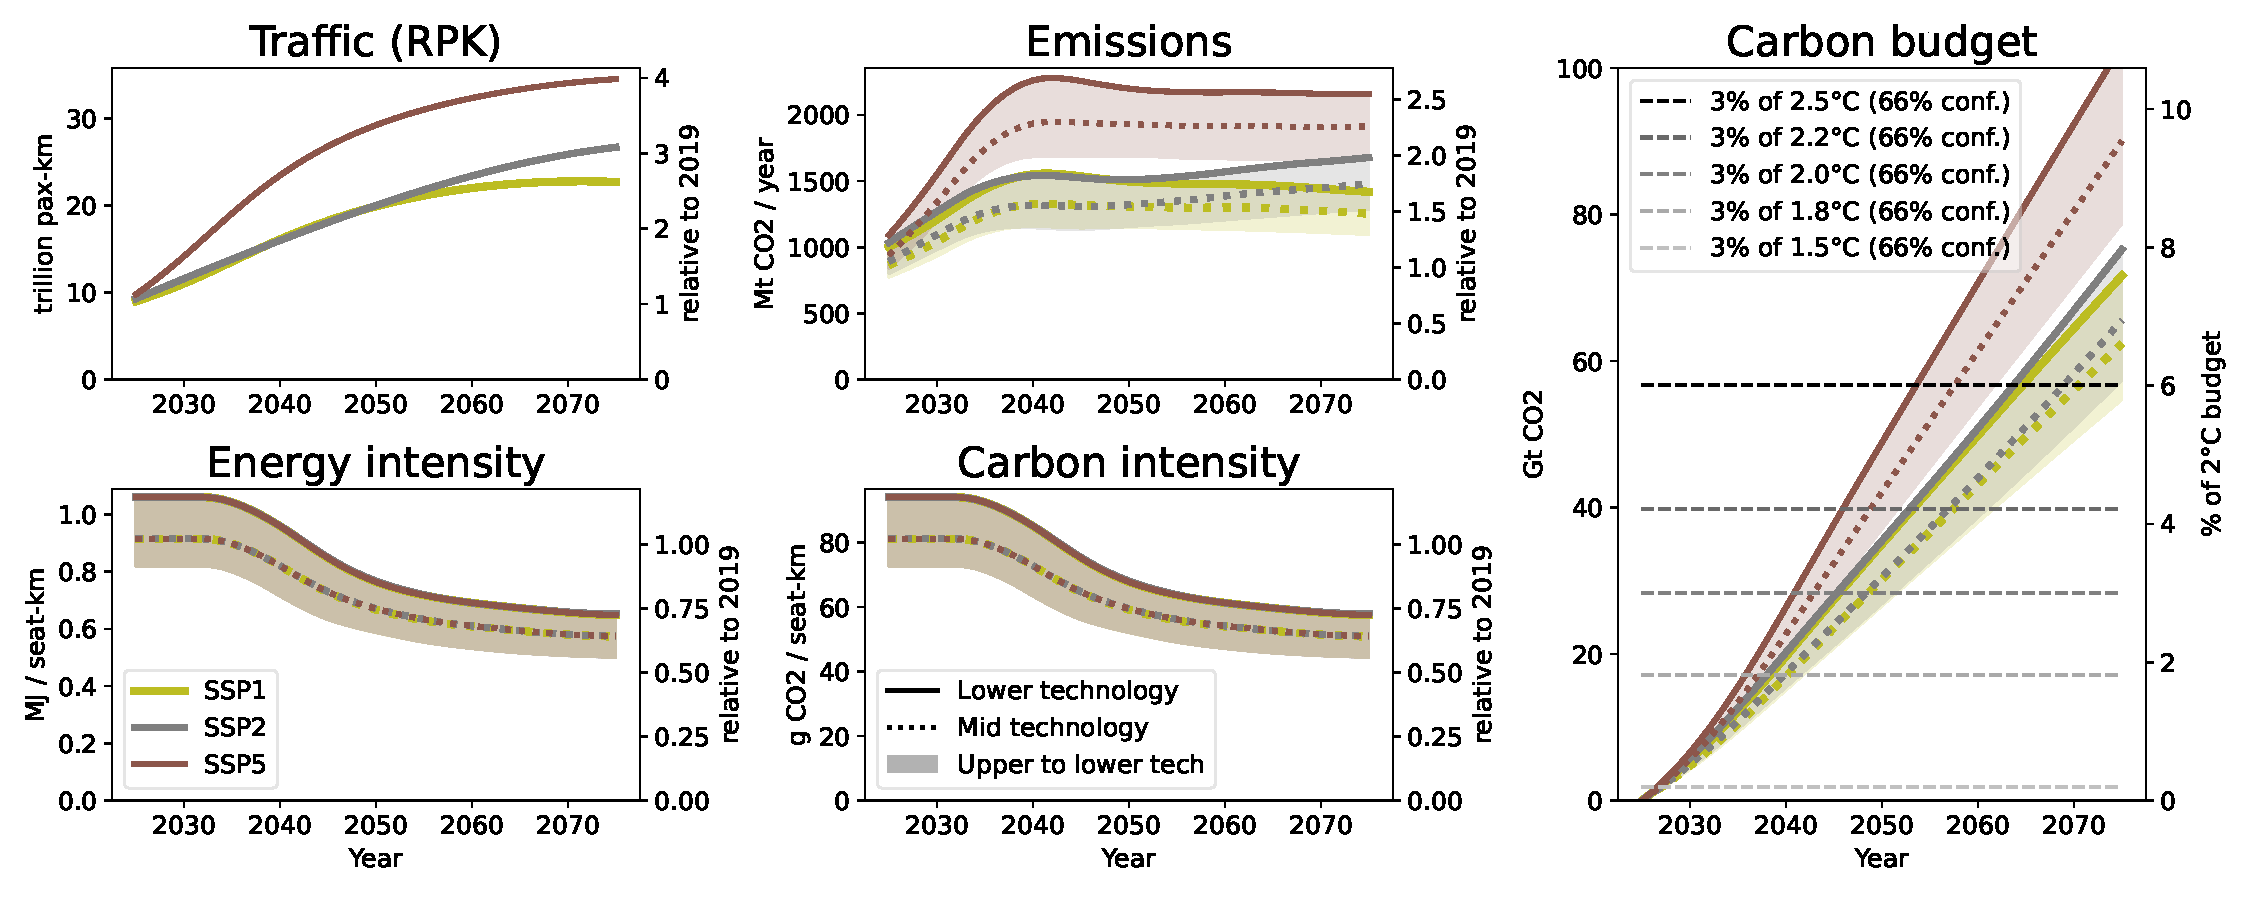
\includegraphics[width=0.85\textwidth]{figs/baseline.pdf}

    (b) Drop-in:

    
\includegraphics[width=0.85\textwidth]{figs/dropin.pdf}

    (c) Breakthrough:

    
\includegraphics[width=0.85\textwidth]{figs/breakthrough.pdf}
    \caption{Comparison of scenario trends (traffic, annual and cumulative emissions, carbon and energy intensity) for (a) Baseline, (b) Drop-in, and (c) Breakthrough. The sensibility to aircraft technology is displayed with 3 aircraft technology scenarios: Lower (continuous line), Mid (dotted line), and Upper technology (shadowed region).}
    \label{fig:trends}
\end{figure*}

\begin{figure*}
    \centering
    
\includegraphics[width=\textwidth]{figs/fleet_SSP2-26-Fossil-midTech.pdf}
    \caption{Aircraft fleet composition and carbon intensity of supply for each of the market segments, for the no-policy baseline SSP2 scenario with Mid aircraft technology.}
    \label{fig:baseline-fleet}
\end{figure*}

The Breakthrough mitigation scenario increments the Drop-in by introducing new alternative aircraft concepts (Battery-Electric, LH2 Fuel-Cell, and LH2 Gas Turbine), and is also divided into a trend, availability, and low-demand variant, each sweeping the 3 technology scenarios.

Finally, the scenario-robust mitigation scenarios keep all mitigation measures (SAF and deployment of alternative aircraft), but the objective is now to optimize the mean among 3 different background scenarios: SSP2-1.9, 2.6, and 3.4. These scenarios keep the trend assumption of 5.0 \% global energy production allocated to aviation, and are divided into a trend and low-demand variant. For simplification purposes, these are only explored with the Mid aircraft technology.

The overall scenario results are presented and analyzed here, for the presentation of full fleet and energy results refer to the section 2 of the SI.

\subsection{Baseline scenarios}

The emissions in baseline scenarios are mainly driven by the growth in RPK demand, shown in Figure \ref{fig:trends} along with the annual and cumulative CO2 emissions. SSP5 displays the highest initial demand growth, while SSP1 and 2 show close agreement until around 2050, where SSP2 demand continues to grow while SSP1 demand peaks and then declines.

All scenarios are subject to the deployment of new conventional aircraft by 2030, which allows for reducing energy and carbon intensity. Figure \ref{fig:baseline-fleet} breaks down fleet composition and carbon intensity among market segments. Efficiency gains are most pronounced over shorter ranges. The general market for instance can achieve over 3x lower consumption with dedicated aircraft relative to current median commercial flights, however the segment has the longest aircraft lifetimes and accounts for less than 3 \% of global supply. It's in the commuter and regional segments where renewal generates most of the system-wide impacts, due to their moderate-to-high efficiency gains, fast fleet renewal, and higher shares of supply (22 \% and 39 \%, respectively). The short-medium and long-range markets retain substantial shares of current aircraft for longer (slower renewal), but also because it takes time for expected weight reduction targets to perform better than current standards (later EIS).

This leads to annual emissions that are growing until a peak is reached around 2040, where efficiency gains due to aircraft replacement outpace demand growth. However, after the introduction of the first generation of new aircraft, further energy consumption gains with the second generation are only marginal. In SSPs 1 and 5 emissions practically stabilize after the peak due to due to slower pace of demand growth, while continued demand growth in SSP2 result growing emissions after fleet is replaced. All of the baseline scenarios display much higher emission levels compared to the year 2019, around 50 \% higher for SSP1, 80 \% for SSP2, and 120 \% for SSP5.

\begin{figure*}[htbp]
    \centering

    (a) Drop-in:

    
\includegraphics[width=\textwidth]{figs/dropin_jetfuel.pdf}

    (b) Breakthrough:

    
\includegraphics[width=\textwidth]{figs/breakthrough_jetfuel.pdf}
    \caption{Comparison of Jet-A fuel blend for (a) Drop-in, and (b) Breakthrough scenarios. The sensibility to aircraft technology is displayed with 3 scenarios of component-level performances: Lower technology (continuous line), Mid technology (dotted line), and Upper technology (shadowed region). These impact the performance of current and new aircraft designs, as well as the speed of fleet renewal.}
    \label{fig:jet}
\end{figure*}

\begin{figure*}[htbp]
    \centering
    
\includegraphics[width=\textwidth]{figs/breakthrough_carriers.pdf}
    \caption{Comparison of supply per final energy carrier for the Breakthrough mitigation scenarios. The sensibility to aircraft technology is displayed with 3 scenarios of component-level performances: Lower technology (continuous line), Mid technology (dotted line), and Upper technology (shadowed region). These impact the performance of current aircraft, new aircraft, and the speed of fleet renewal, driving the choice of which architectures to deploy and when they are launched.}
    \label{fig:carrier}
\end{figure*}

Cumulative emissions are also much higher than what the considered fair share for aviation. All baseline scenarios exceed its share of contribution to the Paris Agreement target of 2° C by a factor of 2-3, exceeding its share of carbon budget as soon as 2040 in SSP5 and 2046 in SSPs 1 and 2.

\subsection{Mitigation policy optimization}

The outcomes of Drop-in and Breakthrough mitigation are presented in Figure \ref{fig:trends} and compared with the no-policy baseline SSP2.

\begin{figure*}
    \centering

    (a) Breakthrough trend, Lower tech:

    
\includegraphics[clip, trim=0cm 10.6cm 0cm 0cm, width=0.86\textwidth]{figs/fleet_SSP2-26-lowTech.pdf}

    (b) Breakthrough availability, Lower tech:

    
\includegraphics[clip, trim=0cm 10.6cm 0cm 0cm, width=0.86\textwidth]{figs/fleet_SSP2-26-Availability-lowTech.pdf}

    (c) Breakthrough low-demand, Lower tech:

    
\includegraphics[clip, trim=0cm 11cm 0cm 0cm, width=0.86\textwidth]{figs/fleet_SSP2-26-LowDemand-lowTech.pdf}

    (d) Breakthrough trend, Upper tech:

    
\includegraphics[clip, trim=0cm 10.6cm 0cm 0cm, width=0.86\textwidth]{figs/fleet_SSP2-26-upTech.pdf}


    (e) Breakthrough availability, Upper tech:

    
\includegraphics[clip, trim=0cm 10.6cm 0cm 0cm, width=0.86\textwidth]{figs/fleet_SSP2-26-Availability-upTech.pdf}

    (f) Breakthrough low-demand, Upper tech:

    
\includegraphics[clip, trim=0cm 6.2cm 0cm 0cm, width=0.86\textwidth]{figs/fleet_SSP2-26-LowDemand-upTech.pdf}

    \caption{Comparison of aircraft fleet composition per market for a set of simulated mitigation scenarios. Assumptions on energy availability and aircraft technology significantly impacts the performance of new aircraft designs, driving the choice of which architectures to deploy and when they are launched.}
    \label{fig:fleet}
\end{figure*}

Overall, the Drop-in mitigation scenarios are less sensitive to aircraft technology assumptions, as emission reductions is achieved either with SAF incorporation or demand aversion. The trend variant reaches emission levels comparable to 2019, but fails to phase out of consuming fossil fuels. The availability variant further reduces emission levels, and allow for much lower fossil consumption. The low-demand variant, traffic is nearly half of the trend by 2070, but still around 50 \% higher than the 2019 reference, this variant is the only one that allows for keeping the cumulative emissions in check with the Paris Agreement, phasing out of fossil consumption, and lowering the emissions peak.

The Breakthrough mitigation displays much higher sensitivity to aircraft technology, lower emission levels than Drop-in mitigation (when compared with similar technology), and lower fossil consumption. The trend variant, for instance, still consumes fossil fuels and can emit more than 2019 emissions with Lower technology, or less than half of 2019 with Upper technology. The availability variant can reach near zero emissions after 2070, phasing out of fossil can happen as soon as 2060, allowing for relaxing the biomass consumption constraint, but cumulative emissions are still higher than the sector's fair share. The low-demand variant respects the carbon budget constraint with much less difficulty than the Drop-in low-demand, allowing for much higher demand levels, which may reach up to 140 \% more traffic than 2019, but is still lower than the trend 200 \% increase.

Figure \ref{fig:jet} compares how the Jet-A fuel is composed, blending SAF from BtL and PtL into fossil kerosene. Figure \ref{fig:sankey} details further how energy resources are split among production pathways in order to provide for final energy carriers, in a subset of scenarios. Regarding biofuel production, while the HEFA pathway displays significantly higher emissions compared to FT, it consumes significantly less biomass. This yields that, in scenarios where fossil kerosene consumption is still high, biomass is preferentially allocated to HEFA production. For electrofuel production, Breaktrough scenarios display much lower shares of electrofuel in the Jet-A blend, because hydrogen and electricity are preferentially allocated to alternative aircraft rather than to make electrofuel, but this trade-off is highly dependent on the flight distance considered.

\begin{figure*}[htbp]
    \centering
    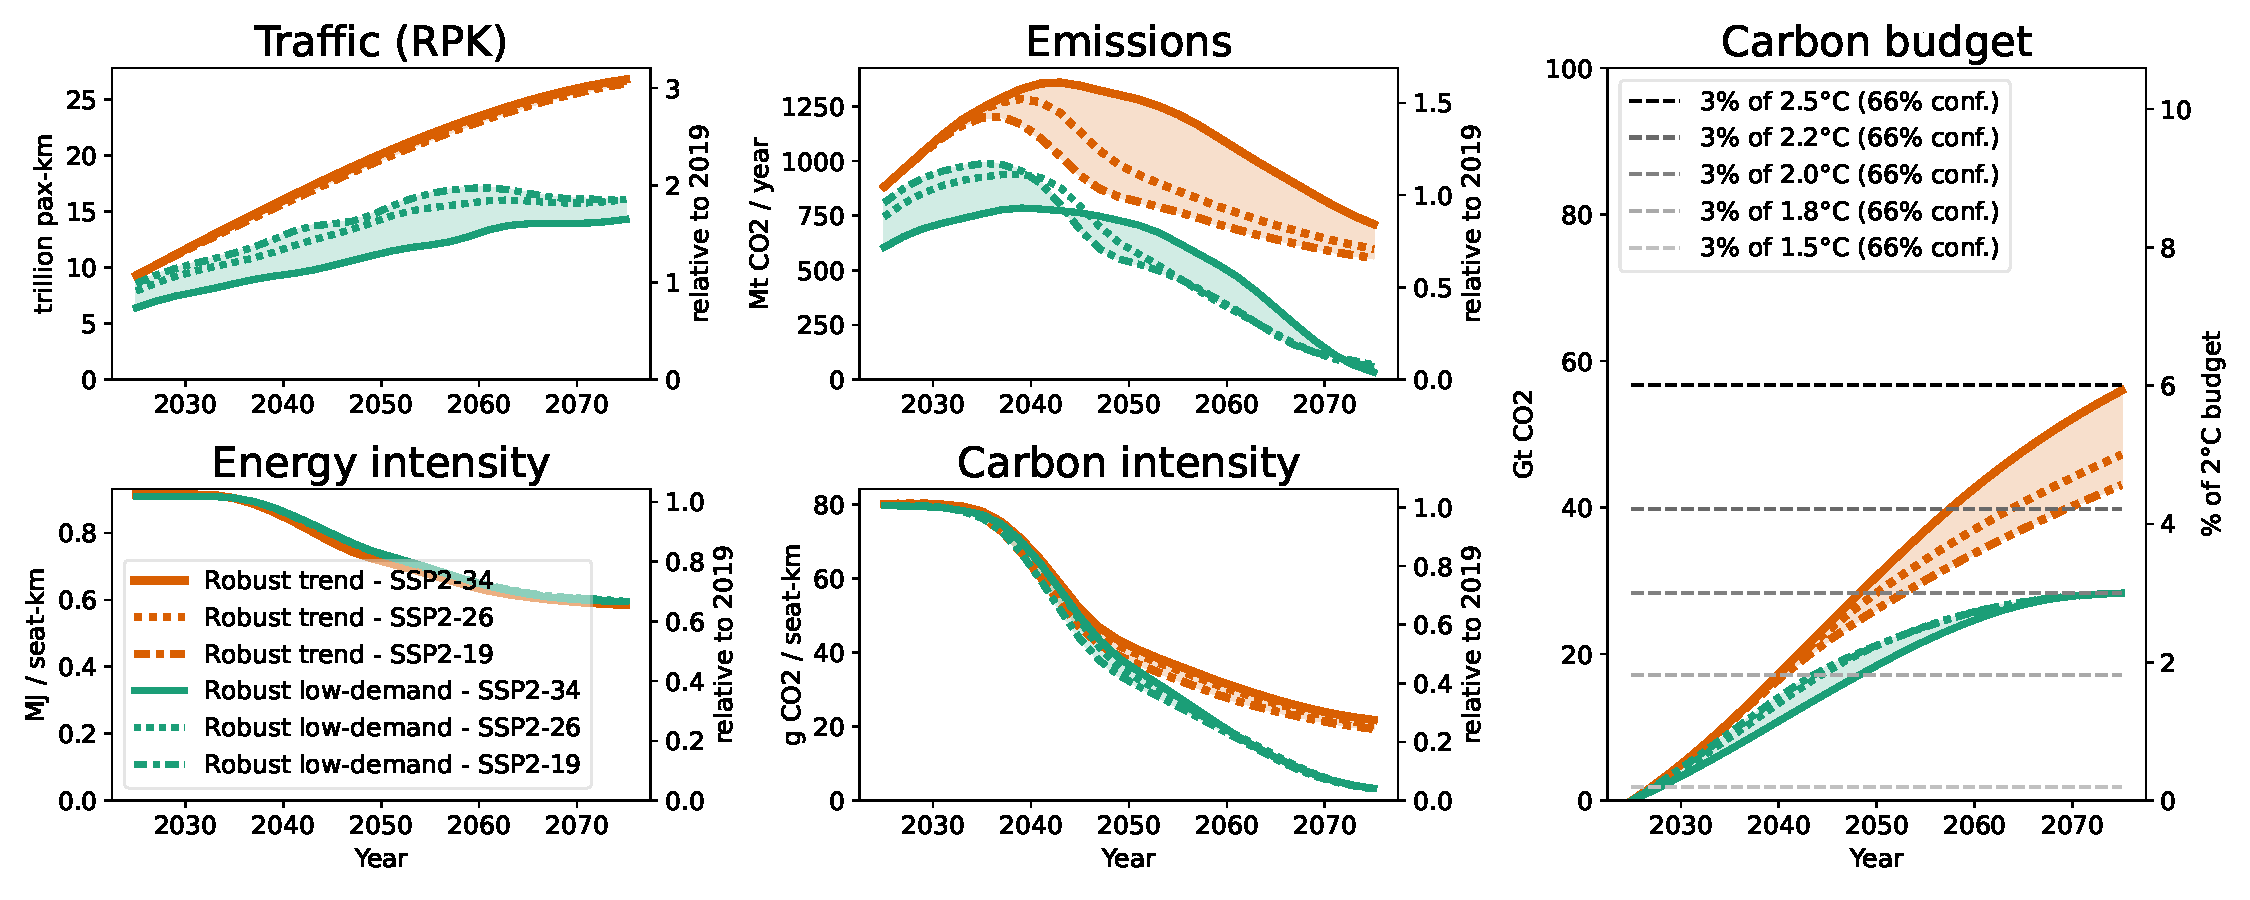
\includegraphics[width=0.9\textwidth]{figs/multi_ensemble_trends.pdf}

    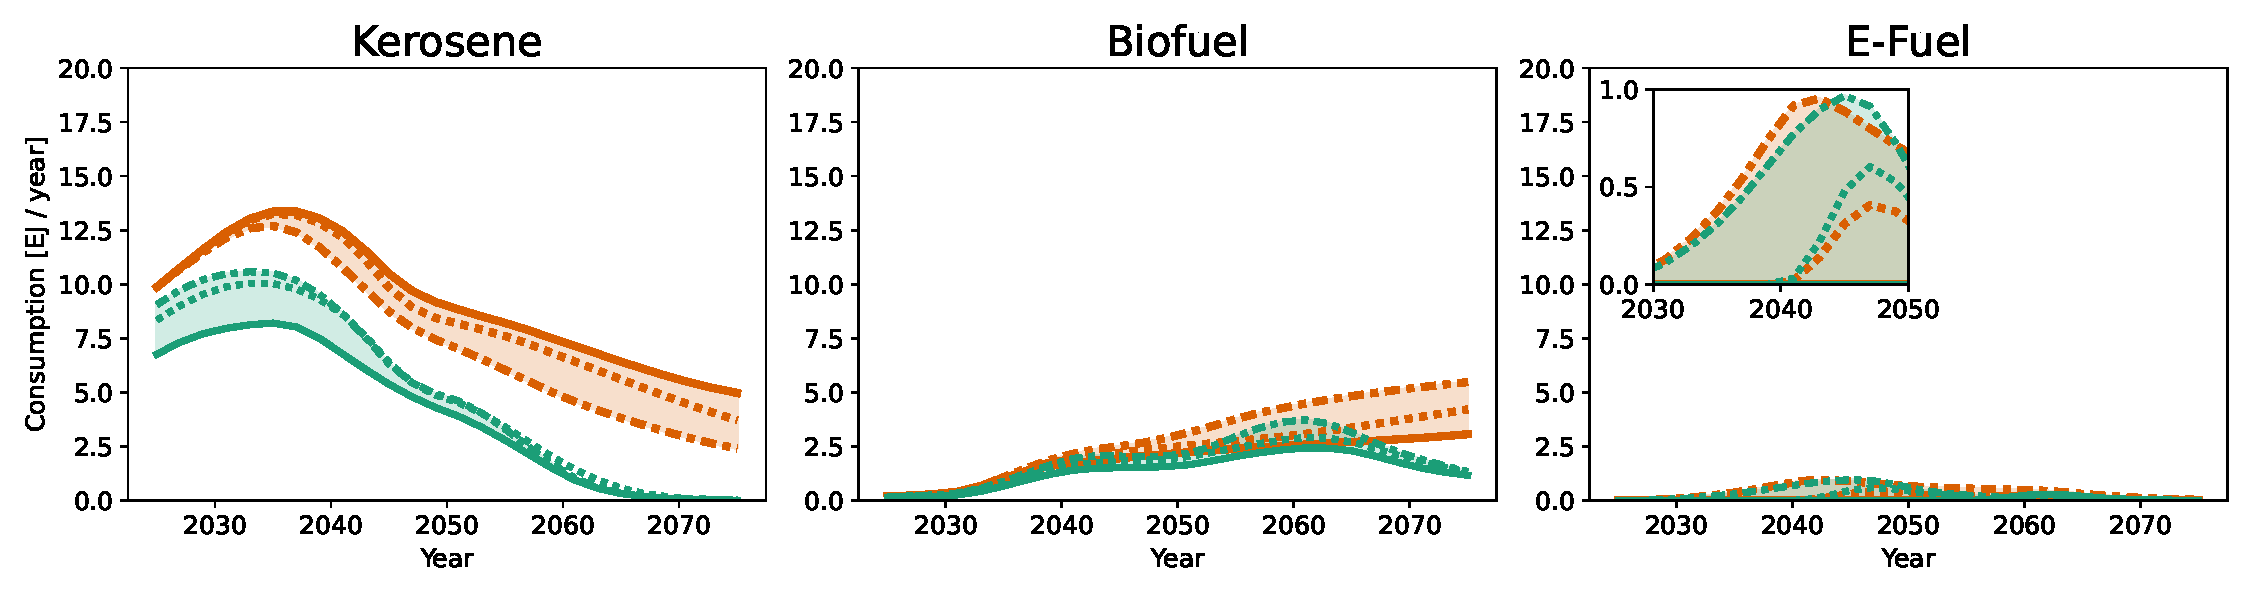
\includegraphics[width=0.95\textwidth]{figs/multi_ensemble_jet_fuel.pdf}

    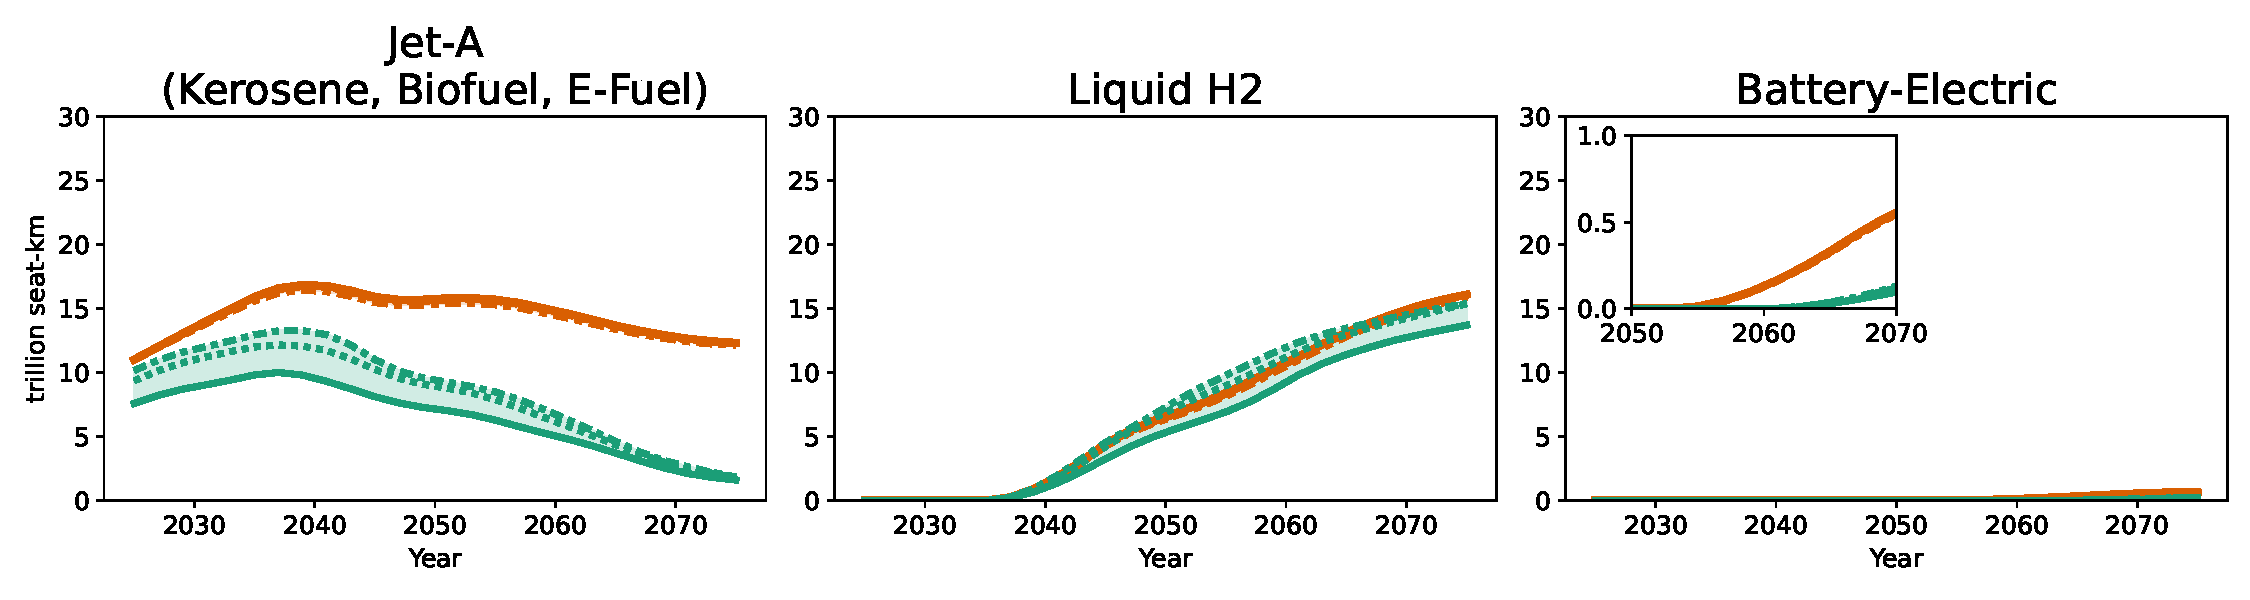
\includegraphics[width=0.95\textwidth]{figs/multi_ensemble_fleet_carriers.pdf}
    \caption{Comparison of trend and low-demand scenario-robust mitigation under Mid aircraft technology and background scenarios SSP2 with RCP's 1.9, 2.6, and 3.4. These strategies prioritizes flexibility by sizing alternative-aircraft deployment for the worst electricity conditions (SSP2-3.4), yielding higher SSP2-2.6 emissions but greater adaptability across SSP2-1.9 and SSP2-3.4.}
    \label{fig:robust}
\end{figure*}

Regarding the aircraft fleet, Figure \ref{fig:carrier} shows the overall comparison of supply according to final energy carrier, while Figure \ref{fig:fleet} provides the bottom-up view of how aircraft technologies are composed to make up the supply in each market segment. The general and commuter markets are consistently the first to transition toward new aircraft, whereas short-medium and long-range markets remain dependent on drop-in fuels for longer periods. The Breakthrough scenarios demonstrate the importance of both technological maturity and availability assumptions: Lower technology delay deployment of hydrogen systems, but once extra energy availability is assumed alternative aircraft are launched as soon as available. In contrast, the Upper technology case allows for more aggressive displacement of conventional aircraft, and also drive the adoption of Battery-Electric in the general market and of Hydrogen Fuel-Cells on remaining markets.

\subsection{Scenario-robust mitigation policy}

As the SSP2-2.6 was chosen as background scenario for the single policy optimization, we include scenarios SSP2-1.9 and SSP2-3.4 in the scenario-robust optimization, to account for different radiative forcing targets, representing a more ambitious and a less ambitious scenario. The outcomes of this multi-scenario policy optimization are shown in Figure \ref{fig:robust}. Compared to the single-scenario optimum, the robust optimum display higher emissions on the target scenario SSP2-2.6, yet it allows for greater flexibility in the case an adjacent global scenario takes place. Overall, this is due to smaller shares of alternative aircraft, driven by the strong difference in the availability of electricity and emission factor associated to grid electricity among the scenarios. The overall strategy is to use the worst case scenario (higher electricity emission factor and less electricity availability) to determine the deployment of alternative aircraft, and use the surplus electricity in the other scenarios to make extra electrofuels for conventional aircraft, leaving room for more variability.

Among these three scenarios, lower warming levels lead to: earlier deployment of electrofuels due to lower electricity emission factor, higher shares of electrofuel due to the higher electricity availability, higher shares of FT pathway in the biofuel blend, and higher shares of biofuel in the Jet-A blend.

\subsection{Comparison with literature}

\begin{figure*}
    \centering
    
\includegraphics[width=\textwidth]{figs/ar6_comparison.pdf}
    \caption{Comparison of aviation final energy demand and direct CO2 emissions between the scenarios developed in this work and the AR6 scenario ensemble \cite{ar6_database}. The AR6 shaded envelope reflects diverse assumptions across models regarding aviation scope, demand growth, efficiency gains, and fuel transitions. The trajectories from this study remain within the ensemble’s range through mid-century, while the stronger long-term decline results from explicitly modeling per-capita demand saturation and full fleet renewal.}
    \label{fig:comparison}
\end{figure*}

Figure \ref{fig:comparison} contrasts aviation's projected final energy use and emissions from the scenarios generated in this work against the AR6 scenario ensemble. The AR6 ensemble exhibits substantial variation, reflecting divergent modeling assumptions regarding aviation scope (international versus domestic, commercial operations, freight inclusion), demand growth trajectories, efficiency improvements, and alternative fuel adoption pathways. The scenarios developed in this study fall within the inter-model spread of the AR6 ensemble for both energy consumption and CO2 emissions through approximately 2050, demonstrating broadly consistent near- to mid-term dynamics.

Beyond 2050, the present work projects lower energy and emissions compared to much of the AR6 ensemble. This divergence stems primarily from the incorporation of demand saturation effects—as per-capita incomes rise according to SSP narratives, the logistic demand model captures the stabilization of air travel propensity at high income levels, rather than assuming continued growth. This comparison validates the plausibility of the scenarios presented in this work, as they remain consistent with the AR6 range while providing additional insight through explicit modeling of demand saturation dynamics, technology-specific aircraft performance, and resource constraints.

\section{Discussion}
\label{sec:discus}

Considering trend traffic growth and allocation of energy resources, even with optimistic technological breakthrough, aviation share of emissions will grow as the wider economy decarbonizes in a 2°C temperature increase scenario. This is in line with scenarios from the IPCC's 6th Assessment Report \cite[][Figure 3.19]{long_ar6_wg3}, in which transport emissions take the longest to reach net zero even in scenarios below 1.5°C with little overshoot.

Regarding the implications for the energy system, fulfilling aviation's needs will require significant volumes of low-carbon electricity and biomass. Limited production amounts will require dedicated policy on which sectors to prioritize the access to these resources. These findings are also in line with recent studies focused on the aviation sector \cite{becken_implications_2023, eaton_regional_2024, drunert_ptl}. Dedicated production facilities integrated near airports might be a way to reducing associated supply chain losses and costs \cite{hoelzen_h2-powered_2025}.

As the efficiencies of energy conversion processes can vary strongly depending on the primary energy source, their comparison must be made on a per unit of service basis. While some studies on several transport modes \cite{wallington_green_2024} consider the base service unit as 1 MJ of thrust (or to wheels), this work instead, considers it to be a traffic measure (passenger-kilometer). This distinction is fundamental for aviation due to the different weights of the propulsion architectures to power these vehicles.

Air transportation is highly unequal sector, both across (see Figure 3 in SI) and within \cite{GOSSLING2020102194} countries. Given that most of the traffic growth in the next decades will happen in emerging economies, which have not yet reached demand saturation. Many of these, however, are still steering public policy to increase access to air travel, e.g., \cite{voa-brasil}. The public acceptance and effectiveness of demand-side measures can be questioned, and using pricing mechanisms to address this problem also raises questions of social justice \cite{Buchs02012024}.

Also, climate change is but one within the Planetary Boundaries \cite{rockstrom_safe_2009, richardson_earth_2023}. Some recent assessments that expand the scope for other Planetary Boundaries \cite{pais_current_2024} stress on the need for acknowledging other limits to avoid shifting the problem, such as biodiversity loss and eutrophication of freshwater ecosystems, especially when considering a strong uptake of biofuels, which are present in most of the industry decarbonization roadmaps \cite{becken_implications_2023}.

Finally, given a set of technology forecasts, optimization can be useful for deciding which technologies to prioritize and when, especially when they compete for similar resources. Yet, in many IAM applications that use optimization, the formulation of the optimization problem is often left unchanged or is little discussed, even if the choice of policy goal (objective) and non-negotiables (constraints) are a fundamental part of the process.

\section{Conclusion}
\label{sec:conclus}

Overall results show that, under trend demand growth: baseline scenarios display a peak in emissions between 2035 and 2040, mitigation scenarios based solely on SAF has limited emissions reductions due to energy availability constraints (2070 emissions are still 75 \% of 2019 with preferential availability), breakthrough aircraft technologies can allow for reaching near zero emissions, but their impact is delayed to after 2045 due to late Entry-Into-Service and slow fleet renewal.

The choice of which aircraft architecture and energy carrier to embark is highly dependent on vehicle performance (determined by TLAR and technology assumptions) and on the background energy system (due to the timing of electricity decarbonization and to limited availability of electricity and biomass).

In order to respect Paris Agreement targets under an effort-sharing principle, drop-in mitigation will put the system to a higher stress: either by constraining traffic, or by consuming too much biomass and electricity. New aircraft with alternative energy carriers allows to reduce such stress by making better use of the same energy resources, even if their energy consumption is higher than that of conventional planes.

When comparing mitigation policies with different objective functions, it was found that supply caps, energy availability, and the introduction of alternative aircraft designs are complementary rather than competing measures. One strategy alone can achieve reduction in emissions up to a certain level, but their combined use is capable of more efficient mitigation by: using alternative aircraft in its feasible markets (reducing needs for low-carbon electricity and biomass for a given service), and avoiding emission-intense markets (further reducing consumption of fossil kerosene).

Regarding the numerical methods, the use of GEMSEO-JAX allowed for both reducing implementation burden and execution time for the optimization of mitigation scenarios. The simulation of these optimization-based policy scenarios was prohibitive without the speedups obtained, which are of two orders of magnitude at the scenario optimization level and three orders of magnitude at the scenario computation and linearization level.

Our research offers practical insights on how to efficiently use optimization algorithms for mitigation scenarios. Applying these methods for the aviation sector, also shed light on how to optimally allocate aircraft architectures, energy resources, and demand-side measures to achieve stringent mitigation targets.

\section*{Code availability}

All the scripts and data required to reproduce the results from this work are openly available in \url{https://gitlab.com/ian.costa-alves1/noads}.

\section*{Acknowledgements}

Gratitude is extended to the Conceptual Airplane Design and Operations (CADO) team at École Nationale de l'Aviation Civile (ENAC), to the Aviation, Climate, Environment (ACE) group at ISAE-SUPAERO, and to the Institute for Sustainable Aviation (ISA) for their support, assistance, and fruitful discussions. The Generic Aircraft Design Model (GAM), provided by the CADO team, was essential for enabling modeling and analysis of alternative aircraft designs. The AeroMAPS platform, developped by ISAE-SUPAERO and ISA, was reponsible for laying the groundwork upon which this research was built. Special thanks to Pascal Roches, Nicolas Monrolin, Thomas Planès, Scott Delbecq, Antoine Salgas, Florian Simatos, Laurent Joly, and Xavier Carbonneau for their sharp insights, support, and collaboration.

Also, the authors thank the Multidisciplinary Optimization Competence Center at IRT Saint Exupéry, for their availability and support with the methodological developments that preceded this research. Special thanks to Matthias De Lozzo, and Antoine Dechaume for their aid with repository maintenance and thorough code reviews.

\section*{CRediT authorship contribution statement}

\textbf{Ian Costa-Alves}: Writing – original draft, Writing – review \& editing, Conceptualization, Data curation, Investigation, Methodology, Software, Validation, Visualization.

\textbf{Nicolas Gourdain}: Writing – original draft, Writing – review \& editing, Conceptualization, Methodology, Funding acquisition, Project administration, Supervision.

\textbf{François Gallard}: Writing – original draft, Writing – review \& editing, Conceptualization, Methodology, Software, Supervision.

\textbf{Anne Gazaix}: Writing – review \& editing, Conceptualization, Funding acquisition, Project administration, Supervision.

\textbf{Yri-Amandine Kambiri}: Writing – review \& editing, Software, Validation.

\textbf{Thierry Druot}: Writing – review \& editing, Conceptualization, Software, Supervision, Validation.

\section*{Funding sources}

This work was supported by the Occitania region, ISAE-SUPAERO, and IRT Saint Exupéry.

%% Loading bibliography style file
% \bibliographystyle{model1-num-names}
% \bibliographystyle{cas-model2-names}
\bibliographystyle{elsarticle-num}

% Loading bibliography database
\bibliography{cas-refs}

\end{document}
